\chapter{Negotiation}
\label{cha:negotiation}

A negotiation problem is one where multiple agents try to come to an
agreement or \td{deal}. Each agent is assumed to have a preference
over all possible deals.  The agents send messages to each other in
the hope of finding a deal that all agents can agree on. These agents
face an interesting problem. They want to maximize their own utility
but they also face the risk of a break-down in negotiation, or
expiration of a deadline for agreement. As such, each agent must
negotiate carefully, trading off any utility it gains from a tentative
against a possibly better deal or the risk of a breakdown in
negotiation.

decide whether the current deal is good enough or whether it should
ask for more and risk agreement failure.

Automated negotiation can be very useful in multiagent systems as it
provides a distributed method of aggregating distributed knowledge.
That is, in a problem where each agent has different local knowledge
negotiation can be an effective method for finding the one global
course of action which maximizes utility without having to aggregate
all local knowledge in a central location. In fact, the metaphor of
autonomous agents cooperating in this manner to solve a problem that
cannot be solved by any one agent, due to limited abilities or
knowledge, was the central metaphor from which the field of
distributed artificial intelligence, later known as multiagent
systems, emerged \cite{davis83a}. The metaphor is based on the
observation that teams of scientists, businesses, citizens, and others
regularly negotiate over future courses of action and the result of
these negotiations can incorporate more knowledge than any one
individual possesses \cite{surowiecki05a}. \mc{See \cite{squyres05a}
  for the full story on the MER mission to Mars. An exciting read.}
For example, in a NASA rover mission to Mars the various engineering
teams and science teams negotiate over what feature to include in the
rover. The scientists are concerned with having the proper equipment
in Mars so that they can do good science while the engineers try to
ensure that everything will work as expected. Often it is the case
that one side does not understand exactly why the other wants or
rejects a particular feature but by negotiating with each other they
arrive at a rover that is engineered solidly enough to survive the
trip to Mars and has enough equipment to do useful science while
there. Thus, negotiation results in the aggregation of knowledge from
multiple individuals in order to make decisions which are better, for
the whole, than if they were made by any one individual.


\section{The Bargaining Problem}

A specific version of the negotiation problem has been studied in game
theory. It is known as the \td{bargaining problem} \cite{nash50a}.  In
the bargaining problem, we say that each agent $i$ has a utility
function $u_i$ defined over the set of all possible deals $\Delta$.
That is, $u_i: \Delta \rightarrow \Re$. We also assume that there is a
special deal $\delta^-$ which is the no-deal deal.  Without loss of
generality we will assume that for all agents $u_i(\delta^-) = 0$ so
that the agents will prefer no deal than accepting any deal with
negative utility. The problem then is finding a protocol $f$ which
will lead the agents to the best deal. \mc{See \cite[Chapter
  7]{osborne99a} or \cite{osborne90a} for a more extended introduction
  to bargaining.}  But, as with all the game theory we have studied,
it is not obvious which deal is the best one. Many solutions concepts
have been proposed. We provide an overview of them in the next sections.

\subsection{Axiomatic Solution Concepts}
\label{sec:axiom-solut-conc}

An \td{axiomatic} solution concept is one which we can formally
describe and then simply declare it to be our most desirable solution
concept simply because we believe it satisfies all the important
requirements. There are many possible requirements we might want to
impose on a possible solution deal. The most obvious one is Pareto
optimality.

\begin{definition}[Pareto optimal]
  \label{def:pareto-optimal}
  A deal $\delta$ is Pareto optimal if there is no other deal such
  that everyone prefers it over $\delta$. That is, there is no
  $\delta'$ such that \[\forall_i u_i(\delta') > u_i(\delta).\]
\end{definition}
This is an obvious requirement because if a deal is not Pareto optimal
then that means that there is some other deal which all of the agents
like better. As such, it does not make sense to use the non-Pareto
deal when we could find this other deal which everyone prefers.

With only two agents, $i$ and $j$, we can visualize the set of
Pareto-optimal deals by using an $xy$-plot where the $x$ and $y$
coordinates are the utilities each agent receives for a deal. Each
deal then becomes a point in the graph, as seen in
figure~\ref{fig:paretofrontier}.  The \td{pareto frontier} is
represented by the line shown in the upper-right which connects all
the Pareto deals.

We might also want a solution that remains the same regardless of the
magnitude of an agent's utility values.

\begin{SCfigure}
  \begin{minipage}{1.0\linewidth}
    \begin{center}
      \begin{tikzpicture}[style=dstyle]
    \draw[->] (0,0) -- (0,5);
    \draw[->] (0,0) -- (7,0);
    \draw (3.5, -.5) node {$u_i(\delta)$}
    (-1,2.5) node {$u_j(\delta)$};
    \foreach \position in {(1,1), (2,2), (3,3), (4,2.5), 
      (1.4,2), (4,1.7), (3,2.4), (3.1,.8),
      (2.1,1), (.5,2.3), (5.5,.77), (2.3,2.7), (4.9,1.5), (1.8,3.3)}
    \draw[fill] \position node[circle,fill,inner sep=1.5pt] {};
    \draw[gray] (.5,4) node[circle,fill,inner sep=1.5pt,color=black] {}
    -- (2.5,3.7) node[circle,fill,inner sep=1.5pt,color=black] {}
    -- (3,3) node[circle,fill,inner sep=1.5pt,color=black] {}
    -- (4.3,2.8) node[circle,fill,inner sep=1.5pt,color=black] {}
    -- (4.9,1.5) node[circle,fill,inner sep=1.5pt,color=black] {}
    -- (5.5,.77) node[circle,fill,inner sep=1.5pt,color=black] {}
    -- (6.1,.3) node[circle,fill,inner sep=1.5pt,color=black] {};
  \end{tikzpicture}
    \end{center}
  \end{minipage}

\caption{The dots represent possible deals. The deals on the gray line
  are Pareto optimal. The line is the Pareto frontier.}
  \label{fig:paretofrontier}
\end{SCfigure}

\begin{definition}[Independence of utility units]
  \label{def:iuu}
  A negotiation protocol is independent of utility units if when given
  $U$ it chooses $\delta$ and when given $U' =\{(\beta_1
  u_1,\ldots,\beta_I u_I): u \in U\}$ it chooses $\delta'$ where
  \[\forall_i \; u_i(\delta') = \beta_i u_i(\delta).\]
\end{definition}
That is, if an agent in a protocol that is independent of utility
units used to get a utility of 10 from the result deal and now has
multiplied its utility function by 5 then that agent will now get a
utility of 50 from the new resulting deal. So, the utilities the
agents receive remain proportional under multiplication.

\begin{definition}[Symmetry]
  \label{def:symmetric}
  A negotiation protocol is symmetric if the solution remains the same
  as long as the set of utility functions $U$ is the same, regardless
  of which agent has which utility.
\end{definition}
That is, if two agents swapped utility function then they also end up
swapping the utilities they get from the resulting deal. In other
words, the specific agents do not matter, the only thing that matters
are the utility functions.

\begin{definition}[Individual rationality]
  \label{def:individual-rationality}
  A deal $\delta$ is individually rational if \[\forall_i \;
  u_i(\delta) \geq u_i(\delta^-).\]
\end{definition}
So, a deal is individual rational if $u_i(\delta) \geq 0$ since we
will be assuming that $u_i(\delta^-) = 0$. That is, a deal is
individually rational if all the agents prefer it over not reaching an
agreement.

\begin{definition}[Independece of irrelavant alternatives]
  \label{def:iia}
  A negotiation protocol is independent of irrelevant alternatives if
  it is true that when given the set of possible deals $\Delta$ it
  chooses $\delta$ and when given $\Delta' \subset \Delta$ where
  $\delta \in \Delta'$ it again chooses $\delta$, assuming $U$ stays
  constant.
\end{definition}
That is, a protocol is independent of irrelevant alternative if the
deal it chooses does not change after we remove a deal that lost. Only
removal of the winning deal changes the deal the protocol chooses.

Given these requirements we can now consider various possible
solutions to a negotiation problem. In the \td{egalitarian solution}
the gains from cooperation are split equally among the agents. That
is, the egalitarian deal is the one where all the agents receive the
same utility and the sum of their utilities is maximal, that is
\begin{equation}
  \label{eq:n-egalitarian}
  \delta = \arg \max_{\delta' \in E} \sum_i u_i(\delta')
\end{equation}
where $E$ is the set of all deals where all agents receive the same
utility, namely
\[
E = \{ \delta \,|\, \forall_{i,j} u_i(\delta) = u_j(\delta)\}. \] 

\mc{\textbf{egalitarian} n: one who believes in the equality of all
  people.} We can find the egalitarian solution visually for the two
agent case by simply drawing the line $y=x$ and finding the deal on
this line that is farther away from the origin, as seen in
figure~\ref{fig:egalitarian}. Note that the egalitarian deal in this
case is not Pareto optimal. However, if we allowed all possible deals
(the graph would be solid black as every pair of $x,y$ coordinates
would represent a possible deal) then the egalitarian deal would also
be a Pareto deal. Specifically, it would be the point on the $y=x$
line which marks the intersection with the Pareto frontier. Also note
that the egalitarian deal does not satisfy the independence of utility
units requirement since it assumes the utility units for the agents
are comparable, in fact, it assumes that all agents' utility functions
use the same units.

A variation on the pure egalitarian deal is the \td{egalitarian social
  welfare} solution which is the deal that maximizes the utility
received by the agent with the lowest utility. That is, it is the deal
$\delta$ that satisfies
\begin{equation}
  \label{eq:eqalitarian-sw}
  \delta = \arg \max_{\delta} \min_{i} u_i(\delta).
\end{equation}
The egalitarian social welfare solution is especially useful in
scenarios where no deal exists which provides all agents with the same
utility since every problem is guaranteed to have an egalitarian
social welfare solution. However, the solution itself can in some
cases seem very un-egalitarian. For example, a deal where two agents
receive utilities of 10 and 100 respectively is the egalitarian social
welfare solution even when another deal exists which gives the agents
9 and 11 respectively.

\begin{SCfigure}
  \begin{minipage}{1.0\linewidth}
    \begin{center}
  \begin{tikzpicture}[style=dstyle]
    \draw[->] (0,0) -- (0,5);
    \draw[->] (0,0) -- (7,0);
    \draw (3.5, -.5) node {$u_i(\delta)$}
    (-1,2.5) node {$u_j(\delta)$};
    \foreach \position in {(1,1), (2,2), (3,3), (4,2.5), 
      (1.4,2), (4,1.7), (3,2.4), (3.1,.8),
      (.5,4), (2.5,3.7), (4.3,2.8), (6.1,.3),
      (2.1,1), (.5,2.3), (5.5,.77), (2.3,2.7), (4.9,1.5), (1.8,3.3)}
    \draw[fill] \position node[circle,fill,inner sep=1.5pt] {};
    \draw[gray,->] (0,0) {}
    -- (1,1) node[circle,fill,inner sep=1.5pt,color=black] {}
    -- (2,2) node[circle,fill,inner sep=1.5pt,color=black] {}
    -- (3,3) node(a)[circle,fill,inner sep=1.5pt,color=black] {}
    -- (5,5) node[color=black,right] {$y=x$};
    \draw[->] (4.5,2) node[right] {Egalitarian deal} -- (a);
    \draw[fill] (4,3.5) node(b)[circle,fill,inner sep=1.5pt] {};
    \draw[fill] (4,3.5) node(b)[circle,fill,inner sep=1.5pt] {};
    \draw[->] (4.5,3) node[right] {Egalitarian social welfare deal}
    -- (b);
    \draw[dashed,->] (3.5,3.5) -- (7,3.5); 
    \draw[dashed,->] (3.5,3.5) -- (3.5,5); 

  \end{tikzpicture}
    \end{center}
  \end{minipage}
  \caption{Egalitarian and egalitarian social welfare deals. The
    egalitarian social welfare deal can be found by moving the
    perpendicular dashed lines from a point high in the $y=x$ line down to
    $0,0$ until they touch the first deal.}
  \label{fig:egalitarian}
\end{SCfigure}

The \td{utilitarian solution} is the deal that maximizes the sum of
the utilities, that is
\begin{equation}
  \label{eq:n-utilitarian}
  \delta = \arg \max \sum_i u_i(\delta).
\end{equation}
The utilitarian deal is, by definition, a Pareto optimal
deal. There might be more than one utilitarian deals in the case of a
tie. The utilitarian deal violates the independence of utility units
assumption as it also assumes utilities are comparable. 

\mc{\textbf{utilitarian} n : someone who believes that the value of a
  thing depends on its utility.}  We can find the utilitarian deal
visually for the two agent case by drawing a line with slope of $-1$
and, starting at the top right, moving it perpendicular to $y=x$ until
it intersects a deal. The first deals intersected by the line are
utilitarian deals, as shown in figure~\ref{fig:utilitarian}.

\begin{SCfigure}
  \begin{minipage}{1.0\linewidth}
    \begin{center}
      \begin{tikzpicture}[style=dstyle]
    \draw[->] (0,0) -- (0,5);
    \draw[->] (0,0) -- (8.2,0);
    \draw (3.5, -.5) node {$u_i(\delta)$}
    (-1,2.5) node {$u_j(\delta)$};
    \foreach \position in {(1,1), (2,2), (3,3), (4,2.5), 
      (1.4,2), (4,1.7), (3,2.4), (3.1,.8),
      (.5,4), (2.5,3.7), (6.1,.3),
      (2.1,1), (.5,2.3), (5.5,.77), (2.3,2.7), (4.9,1.5), (1.8,3.3)}
    \draw[fill] \position node[circle,fill,inner sep=1.5pt] {};
    \draw[gray,->] (0,0) {}
    -- (1,1) node[circle,fill,inner sep=1.5pt,color=black] {}
    -- (2,2) node[circle,fill,inner sep=1.5pt,color=black] {}
    -- (3,3) node[circle,fill,inner sep=1.5pt,color=black] {}
    -- (5,5) node[color=black,right] {$y=x$};
    \draw[gray] (7.1,0) -- (2,5.1);
    \draw[gray] (8,0) -- (3,5);
    \draw[fill] (4.3,2.8) node[circle,fill,inner sep=1.5pt] (a) {};
    \draw[->] (5,3.5) node[right] {Utilitarian deal} 
    -- (a);
  \end{tikzpicture}
\end{center}
  \end{minipage}
\caption{Utilitarian deal. The line $y = b - x$ starts with a very
  large $b$ which is reduced until the line intersects a deal.}
  \label{fig:utilitarian}
\end{SCfigure}

The utilitarian and egalitarian solutions both seem like fairly
reasonable solutions. Unfortunately, both violate the independence of
utility units assumption. It was Nash who proposed a solution which
does not violate this assumption. The \td{Nash bargaining solution} is
the deal that maximizes the product of the utilities. That is,
\begin{equation}
  \label{eq:n-nash}
  \delta = \arg \max_{\delta'} \prod u_i(\delta').
\end{equation}
The Nash solution is also Pareto efficient
(Definition~\ref{def:pareto-optimal}), independent of utility units
(Definition~\ref{def:iuu}), symmetric
(Definition~\ref{def:symmetric}), independent of irrelevant
alternatives (Definition~\ref{def:iia}).  In fact, it is the
\emph{only} solution that satisfies these four requirements
\cite{nash50a}. This means that if we want a solution that satisfies
these four requirements then our only choice is the Nash bargaining
solution.

\begin{SCfigure}
  \begin{minipage}{1.0\linewidth}
    \begin{center}
      \begin{tikzpicture}[style=dstyle,domain=.01:8]
    \draw[->] (0,0) -- (0,5);
    \draw[->] (0,0) -- (8.2,0);
    \draw (3.5, -.5) node {$u_i(\delta)$}
    (-1,2.5) node {$u_j(\delta)$};
    \foreach \position in {(1,1), (2,2), (3,3), (4,2.5), 
      (1.4,2), (4,1.7), (3,2.4), (3.1,.8),
      (.5,4), (2.5,3.7), (6.1,.3),
      (2.1,1), (.5,2.3), (5.5,.77), (2.3,2.7), (4.9,1.5), (1.8,3.3)}
      \draw[fill] \position node[circle,fill,inner sep=1.5pt] {};

    \draw[gray,->] (0,0) {}
    -- (1,1) node[circle,fill,inner sep=1.5pt,color=black] {}
    -- (2,2) node[circle,fill,inner sep=1.5pt,color=black] {}
    -- (3,3) node[circle,fill,inner sep=1.5pt,color=black] {}
    -- (5,5) node[color=black,right] {$y=x$};
    \draw[fill] (4.3,2.8) node[circle,fill,inner sep=1.5pt] (a) {};

    \draw[->] (5,3.5) node[right] {Nash bargaining deal} -- (a);
%does not work entirely. Need to grep 'i' .table.
    \draw[gray, smooth] plot file {negotiation/nb1.table} node[right]
    {\textcolor{black}{$u_i(\delta) \cdot u_j(\delta) = 1$}};

    \draw[gray, smooth] plot file {negotiation/nb5.table} node[right]
    {\textcolor{black}{$u_i(\delta) \cdot u_j(\delta) = 5$}};

    \draw[gray, smooth] plot file {negotiation/nb10.table} node[right]
    {\textcolor{black}{$u_i(\delta) \cdot u_j(\delta) = 10$}};

  \end{tikzpicture}
\end{center}
  \end{minipage}
\caption{Nash bargaining deal.}
  \label{fig:nash-bargaining}
\end{SCfigure}


Figure~\ref{fig:nash-bargaining} shows a visualization of the Nash
bargaining deal. Each curve represents all pairs of utilities that
have the same product, that is, the line $y = c/x$. As we move
northeast, following the line $y=x$, we cut across indifference curves
of monotonically higher products. As such, the last deal to intersect
a curve is the one which maximizes the product of the utilities, so it
is the Nash bargaining solution.

\medskip

Yet another possible solution is to find the deal that distributes the
utility in proportion to the maximum that the agent could get
\cite{kalai75a}. Specifically, let $u_i^*$ be the maximum utility that
$i$ could get from the set of all deals in the Pareto frontier. That
is, the utility that $i$ would receive if he got his best possible
deal from the Pareto frontier. Then, find the deal that lies in the
line between the point $\delta^-$ and the point $(u_i^*,u_j^*)$. This
solution is known as the \td{Kalai-Smo\-ro\-dinsky solution}. If all
deals are possible then this solution is Pareto optimal. However, if
there are only a finite set of possible deals then this solution might
not exist. That is, there might not be a point in the specified line.
This is a serious drawback to the use of the Kalai-Smo\-ro\-dinsky
solution in a discrete setting.  

The Kalai-Smo\-ro\-dinsky solution, like the Nash bargaining solution,
is also independent of utility units requirement. On the other
hand, it is not independent of irrelevant alternatives.

\begin{SCfigure}
  \begin{minipage}{1.0\linewidth}
    \begin{center}
      \begin{tikzpicture}[style=dstyle]
    \draw[->] (0,0) -- (0,5);
    \draw[->] (0,0) -- (8.2,0);
    \draw (3.5, -.5) node {$u_i(\delta)$}
    (-1,2.5) node {$u_j(\delta)$};
    \draw[gray] (6.1,0) node[black,below] {$u_i^*$} -- (6.1,4) node[black,right] {$u_i^*,u_j^*$}
                  (0,4) node[black,left] {$u_j^*$} -- (6.1,4);
    \draw[gray] (0,0) -- (6.1,4);              

    \draw[gray] (.5,4) node[circle,fill,inner sep=1.5pt,color=black] {}
    -- (2.5,3.7) node[circle,fill,inner sep=1.5pt,color=black] {}
    -- (3,3) node[circle,fill,inner sep=1.5pt,color=black] {}
    -- (4.3,2.8) node[circle,fill,inner sep=1.5pt,color=black] {}
    -- (4.9,1.5) node[circle,fill,inner sep=1.5pt,color=black] {}
    -- (5.5,.77) node[circle,fill,inner sep=1.5pt,color=black] {}
    -- (6.1,.3) node[circle,fill,inner sep=1.5pt,color=black] {};

    \draw[fill] (4.3,2.8) node[circle,fill,inner sep=1.5pt] (a) {};
    \draw (6.2,2) node[right] (ks) {Kalai-Smorodinsky deal};
    \draw[->] (ks) -- (a);
  \end{tikzpicture}
\end{center}
  \end{minipage}
\caption{Kalai-Smo\-ro\-dinsky bargaining deal. We only show deals on
  the Pareto frontier.}
  \label{fig:kalai-deal}
\end{SCfigure}


\medskip

There is no general agreement as to which one of these axiomatic
solutions is better. The social sciences try to develop experiments
that will tell us which one of the solutions, if any, is arrived at by
humans engaged in negotiation. Others try to justify some of these
solutions as more fair than others. We, as multiagent designers, will
probably find that all of them will be useful at some point, depending
on the requirements of the system we are building.


\subsection{Strategic Solution Concepts}
\label{sec:strat-solut-conc}

Another way to think about what solution will be arrived at in a
bargaining problem is to formalize the bargaining process, assume
rational agents, and then determine their equilibrium strategies for
their bargaining process. That is, define the solution concept to be
the solution that is reached by automated rational agents in a bargaining
problem.  This method does raise one large obstacle: we need to first
formally define a bargaining process that allows all the same
``moves'' as real-life bargaining. If you have ever haggled over the
price of an item then you know that it is impossible to formalize all
the possible moves of market-vendor. We need a negotiation protocol
that is simple enough to be formally analyzed but still allows the
agents to use most of their moves.

One such model is the \td{Rubinstein's alternating offers} model
\cite{rubinstein82a}. In this model two agents try to reach agreement
on a deal. The agents can take actions only at discrete time steps. In
each time step one of the agents proposes a deal $\delta$ to the other
who either accepts it or rejects it. If the offer is rejected then we
move to the next time step where the other agent gets to propose a
deal. Once a deal has been rejected it is considered void and cannot
be accepted at a later time.  The agents, however, are always free to
propose any deal and to accept or reject any deal as they wish. We
further assume that the agents know each other's utility functions.

The alternating offers models, as it stands, does not have a dominant
strategy. For example, imagine that the two agents are bargaining over
how to divide a dollar. Each agent wants to keep the whole dollar to
itself and leave the other agent with nothing. Under the basic
alternating offers protocol the agents' best strategy is to keep
proposing this deal to the other agent. That is, each agent keeps
telling the other one ``I propose that I keep the whole dollar'' and
the other agent keeps rejecting this proposal. This scenario is not
very interesting.

In order to make it more interesting, we further assume that time is
valuable to the agents. That is, the agents' utility for all possible
deals is reduced as time passes. For example, imagine that instead of
haggling over a dollar the agents are haggling over how to split an
ice cream sundae which is slowly melting and the agents hate melted
ice cream. Formally, we say that agent $i$'s utility at time $t$ for
deal $\delta$ is given by $\lambda_i^t u_i(\delta)$ where $\lambda_i$
is $i$'s discount factor, similarly the utility for $j$ is
$\lambda_j^t u_j(\delta)$. Thus, the agents' utility for every
possible deal decreases monotonically as a function of time with a
discount factor given by $\lambda$. Note that if $\lambda_i = 0$ then
the agent must agree to a deal at time 0 since after that it will
receive a utility of 0 for any deal. Conversely, if $\lambda_i = 1$
then the agent can wait forever without any utility loss.

Furthermore, lets assume that the agents' utilities are linear and
complementary. Specifically, imagine that the deal $\delta$ is simply
a number between 0 and 1 and represents the amount of utility an agent
receives so that $u_i(\delta) = \delta$ and $u_j(\delta) = 1 -
\delta$. In this scenario, it can be shown that a unique subgame
perfect equilibrium strategy exists.

\begin{theorem}[Alternating Offers Bargaining Strategy]
  \label{the-rubin}
  The Rubinstein's alternating offers game where the agents have
  complementary linear utilities has a unique subgame perfect
  equilibrium strategy where 
  \begin{itemize}
  \item agent $i$ proposes a deal
    \[ \delta_i^* = \frac{1 - \lambda_j}{1 - \lambda_i\lambda_j} \]
    and accepts the offer $\delta_j$ from $j$ only if $u_i(\delta_j)
    \leq u_i(\delta_j^*)$,
  \item agent $j$ proposes a deal
    \[ \delta_j^* = \frac{1 - \lambda_i}{1 - \lambda_i\lambda_j} \]
    and accepts the offer $\delta_i$ from $i$ only if $u_j(\delta_i)
    \leq u_j(\delta_i^*)$.
  \end{itemize}
  \cite{rubinstein82a,muthoo99a}.
\end{theorem}

We can understand how these deals are derived by noting that since
both agents have utilities that decrease with time the best deal will
be reached in the first step. That means that each agent must propose
a deal that the other will accept. Specifically, agent $i$ must
propose a deal $\delta_i^*$ such that $u_j(\delta_i^*) = \lambda_j
u_j(\delta_j^*)$ because if it proposes a deal that gives $j$ lower
utility then $j$ will reject it and if it proposes a deal that gives
$j$ higher utility then $i$ is needlessly giving up some of its own
utility. Conversely, $j$ must propose a deal $\delta_j^*$ such that
$u_i(\delta_j^*) = \lambda_i u_i(\delta_i^*)$. We thus have two
equations.

Since $u_i(\delta) = \delta$ and $u_j(\delta) = 1 - \delta$, we can
replace these definitions into the above equations to get
\begin{align}
  1 - \delta_i^* &= \lambda_j(1 - \delta_j^*) \\
  \delta_j^* &= \lambda_i\delta_i^*.
\end{align}

Upon solving these two equations for $\delta_i^*$ and $\delta_j^*$ we
get the equilibrium values from Theorem~\ref{the-rubin}. More
generally, it has been shown that a unique subgame perfect equilibrium
exists even when the utility functions are not linear but are simply
monotonic in $\delta$.

The theorem tells us that the best strategy for these agents is
propose a bid on the first time step which will be accepted by the
other agent. This action makes sense because we know that utilities
only decrease with time so the best possible deal will be had on the
first time step. The value of the proposed deal, on the other hand, is
very interesting. Notice that the deal $i$ proposes depends only on
the agents' discount factor, not on their utility values. The
important thing is how fast each agent loses utility over time.  For
example, notice that if $\lambda_j = 0$ then $i$ will propose
$\delta_i^* = 1$. That is, $i$ will propose to keep all the utility to
himself. Agent $j$ will accept this proposal since he knows that given
that his $\lambda_j = 0$ if he waits for the next time step then he
will receive utility of 0 in every possible deal.

\medskip

Similar techniques have been used to show the existence of equilibrium
in other types of bargaining games \cite{kraus01a}. These games are
all alternating offer games but assume different utility discounts
such as a fixed loss utility function that is reduced by a constant
amount each time and an interest rate utility which models the
opportunity loss, among others. Depending on the type of utility
discount and the type of game, some of these games can be proven to
have a unique perfect equilibrium strategy that involves only one
actions, others have multiple equilibria and thus would require some
other coordination method, and yet others can be shown to be
NP-complete in the time it takes to find the unique equilibrium.  In
general, however, the technique used to solve these bargaining games
is the same.
\begin{enumerate}
\item Formalize bargaining as a Rubinstein's alternating offers games.
\item Generate extended-form game.
\item Determine equilibrium strategy for this game.
\end{enumerate}
In practice, step~3 is often computationally intractable, at least for
the general case of the problem.


\section{Monotonic Concession Protocol}

The simplest negotiation protocol following the Rubinstein's model of
alternating offers is the \td{monotonic concession protocol}. In this
protocol the agents agree to always make a counter offer that is
slightly better for the other agent than its previous offer.
Specifically, in monotonic concession the agents follow the algorithm
shown in figure~\ref{fig:monotonic-concession}.

\begin{SCfigure}
  \begin{minipage}{1.0\linewidth}
\begin{codebox}
  \Procname{$\proc{monotonic-concession}$}
  \li $\delta_i \gets \arg \max_\delta u_i(\delta)$
  \li Propose $\delta_i$
  \li Receive $\delta_j$ proposal
  \li \If $u_i(\delta_j) \geq u_i(\delta_i)$ 
  \li \Then Accept $\delta_j$
  \li \Else $\delta_i \gets \delta'_i$ such that $u_j(\delta'_i)
	  \geq \epsilon + u_j(\delta_i)$ and $u_i(\delta'_i) \geq u_i(\delta^-)$ 
  \End 
  \li \Goto 2
\end{codebox}
  \end{minipage}
\caption{The monotonic concession protocol.}
  \label{fig:monotonic-concession}
\end{SCfigure}

\begin{SCfigure}
  \begin{minipage}{1.0\linewidth}
    \begin{center}
      \begin{tikzpicture}[style=dstyle]
        \draw[<->] (-.5,-1) -- (-.5,6);
        \draw[->] (-.5,0) -- (6.2,0);        
        \draw (3.5, -.5) node {$\delta$} 
              (-.5,2.5) node[left] {Utility};
        \draw (0,5) node [right] {$u_i(\delta)$} -- (6,-1);

        \draw[color=gray] 
        (0,0) -- (6,4) node [right] {\textcolor{black}{$u_j(\delta)$}};

        \draw (0,0) node[circle,fill,inner sep=1.5pt,color=black] (is) {};
        
        \draw (is) node[below]{\textcolor{black}{$\delta_i^1$}}
        -- node {$~~\epsilon$} ++(0,.8) 
        -- ++(1.2,0) node[below]{$\delta_i^2$}
        -- node {$~~\epsilon$} ++(0,.8) 
        -- ++(1.2,0) node[below]{$\delta_i^3$}
        -- node {$~~\epsilon$} ++(0,.8) 
        -- ++(1.2,0) node[above]{$\delta_i^4$};

        \draw[color=gray] 
        (6,-1) node[below]{\textcolor{black}{$\delta_j^1$}} 
        -- node {$~~\epsilon$} ++(0,.8) 
        -- ++(-.8,0) node[below]{$\delta_j^2$}
        -- node {$~~\epsilon$} ++(0,.8) 
        -- ++(-.8,0) node[below]{$\delta_j^3$}
        -- node {$~~\epsilon$} ++(0,.8) 
        -- ++(-.8,0) node[below]{$\delta_j^4$};

      \end{tikzpicture}
    \end{center}
  \end{minipage}
  \caption{Monotonic concession protocol visualization. Both agents
    have linear utility functions over the set of deals. The
    superscripts indicate the time so $\delta_i^1$ is $i$'s proposal
    at time 1. At time 4 we have that $\delta_i^4 = \delta_j^4$ so
    $u_i(\delta_j^4) = u_i(\delta_i^4)$ and the agents agree on this
    deal. }
  \label{fig:monocon}
\end{SCfigure}

%Maybe, show protocol as AUML diagram.

Each agent starts by proposing the deal that is best for itself. The
agent then receives a similar proposal from the other agent. If the
utility the agent receives from the other's proposal is bigger than
the utility it gets from its own proposal then it accepts it and
negotiation ends. If no agreement was reached then the agent must
propose a deal that is at least an increase of $\epsilon$ in the other
agent's utility. If neither agent makes a new proposal then there are
no more messages sent and negotiations fail, so they implicitly agree
on the no-deal deal $\delta^-$. The monotonic concession protocol
makes it easy for the agents to verify that the other agent is also
obeying the protocol. Namely, if $i$ ever receives a proposal whose
utility is less than a previous proposal then it knows that $j$ is not
following the protocol.

The protocol can be visualized as in figure~\ref{fig:monocon}. Here we
see a simple example with linear utility functions where the agents
reach an agreement ($\delta^4$) after four time steps. Notice that the
agreement reached is \emph{not} the point at which the lines
intersect. The monotonic concession protocol is not guaranteed to
arrive at any particular axiomatic solution concept.  All that it
guarantees is that it will stop.

Monotonic concession has several drawbacks. It can be very slow to
converge. Convergence time is dictated by the number of possible
deals, which is usually very large, and the value of $\epsilon$. It is
also impossible to implement this algorithm if the agents do not know
the other agents' utility function. \mc{A common workaround is to
  assume its a zero-sum game and use the agent's own utility
  function.} In practice, it is rare for an agent to know its
opponent's utility function. Finally, the monotonic concession
protocol has a tricky last step. Namely, the two agents could make
simultaneous offers where each one ends up preferring the other
agent's offer to the one it just sent. This is a problem as both of
them now want to accept different offers. This can be solved by
forcing the agents to take turns. But, if we did that then neither
will want to go first as the agent that goes first will end up with a
slightly worse deal.

\subsection{The Zeuthen Strategy}

The monotonic concession protocol we presented implements a simplistic
strategy for the agent: always concede at least $\epsilon$ to the
other agent. However, if an agent knows that the other one will always
concede then it might choose to not concede at all. Smarter agents
will examine their opponent's behavior and concede in proportion to
how much they are conceding.

This idea is formalized in the \td{Zeuthen strategy} for the monotonic
concession protocol. We start by defining the willingness to risk
a breakdown in negotiations to be
\begin{equation}
  \label{eq:6}
  \text{risk}_i = \frac{u_i(\delta_i) - u_i(\delta_j)}{u_i(\delta_i)}.
\end{equation}
The agent can then calculate the risks for both agents. The Zeuthen
strategy tells us that the agent with the smallest risk should concede
just enough so that it does not have to concede again in the next time
step. That is, the agent that has the least to lose by conceding
should concede. More formally, we define the new protocol as shown in
figure~\ref{fig:mcp-zeuthen}.


\begin{SCfigure}
  \begin{minipage}{1.0\linewidth}
    \begin{codebox}
  \Procname{$\proc{zeuthen-monotonic-concession}$}
  \li $\delta_i \gets \arg \max_\delta u_i(\delta)$
  \li Propose $\delta_i$
  \li Receive $\delta_j$ proposal
  \li \If $u_i(\delta_j) \geq u_i(\delta_i)$ 
  \li \Then Accept $\delta_j$
  \End
  \li $\text{risk}_i \gets \frac{u_i(\delta_i) - u_i(\delta_j)}{u_i(\delta_i)}$
  \li $\text{risk}_j \gets \frac{u_j(\delta_j) - u_j(\delta_i)}{u_j(\delta_j)}$
  \li \If $\text{risk}_i < \text{risk}_j$
  \li \Then $\delta_i \gets \delta'_i$ such that
            $\text{risk}_i(\delta'_i) > \text{risk}_j(\delta'_j)$
  \li \Goto 2
  \End
  \li \Goto 3
\end{codebox}
\caption{The monotonic concession protocol using the Zeuthen
  strategy.}
\label{fig:mcp-zeuthen}
  \end{minipage}
\end{SCfigure}


\begin{SCfigure}
  \begin{minipage}{1.0\linewidth}
    \begin{center}
      \begin{tikzpicture}[style=dstyle]
        \draw[<->] (-.1,-1) -- (-.1,5);
        \draw[->] (-.1,0) -- (6.2,0);
        \draw (3.5, -.5) node {$\delta$};
        \draw (3.5, -.5) node {$\delta$} 
              (-.5,2.5) node[left] {Utility};
        \draw (0,5) node [right] {$u_i(\delta) = 5 - \delta$} -- (6,-1);

        \draw[color=gray] 
        (0,0) -- (6,4) node [above] {$u_j(\delta) = \frac{2}{3}\delta$};

        \draw (0,0) node[circle,fill,inner sep=1.5pt,color=black] {};
        \draw (0,0) node[below right] {$\delta_i^0 = 0$};
        \draw (6,0) node[circle,fill,inner sep=1.5pt,color=gray]  {};
        \draw (6,0) node[below] {$\delta_j^0 = 6$};
        \draw (4.9,0) node[circle,fill,inner sep=1.5pt,color=gray]  {}
        (4.9,0) node[circle,fill,inner sep=1.5pt,color=gray]  {}
        (4.9,0) node[above right] {$\delta_j^1 = 4.9$};
      \end{tikzpicture}
    \end{center}
  \end{minipage}
  \caption{Visualization of the Zeuthen strategy at work. The initial
    proposals are $\delta_i^0=0$ and $\delta_j^0=6$.  }
  \label{fig:zeuthen}
\end{SCfigure}

Figure~\ref{fig:zeuthen} shows a graphical representation of the first
step in a Zeuthen negotiation. After the initial proposal the agents
calculate their risks to be
\[\text{risk}_i^0 = \frac{5 - (-1)}{5} = \frac{6}{5}\]
and
\[\text{risk}_j^0=\frac{4 - 0}{4} = 1.\] Since $j$ has a lower risk it
must concede. The new deal must be such that $j$ will not be forced to
concede again. That is, it must insure that
\[\text{risk}_i = \frac{5 - (5 - \delta_j)}{5} < \frac{\frac{2}{3}\delta_j
  - 0}{\frac{2}{3}\delta_j} = \text{risk}_j \] which simplifies to
$\delta_j < 5$. As such, $j$ can pick any deal $\delta$ less than 5.
In the figure the agent chooses $\delta_j^1 = 4.9$.

The Zeuthen strategy is guaranteed to terminate and the agreement it
reaches upon termination is guaranteed to be individually rational and
Pareto optimal.  Furthermore, it has been shown that two agents using
the Zeuthen strategy will converge to a Nash bargaining solution.

\begin{theorem}[Zeuthen converges to Nash solution]
  If both agents use the Zeuthen strategy they will converge to a Nash
  bargaining solution deal, that is, a deal that maximizes the product
  of the utilities \cite{harsanyi65a}.
\end{theorem}
The proof of the theorem shows how the maximum of both agents'
utilities monotonically increases until the protocol reaches an
agreement. As such, if there is any other agreement that has higher
utility than the one they agreed upon then that agreement would have
been proposed in the negotiation. Therefore, there can be no deal with
higher utility for any agent than the one they agreed on.

\medskip

A problem with the Zeuthen strategy might arise in the last step if
the agents' risks are exactly the same. Specifically, if both agents
realize that their risks are the same and that the next proposal that
either of them makes will be accepted by their opponent then both
agents will want to wait for the other agent to concede. This is an
example of the game of chicken. As such, selfish agents should play
the Nash equilibrium strategy which, in this case, is a mixed
strategy. Since it is a mixed strategy it means that there remains a
possibility for both of them to decide to wait for the other one,
thereby breaking down the negotiations when a solution was possible.

The Zeuthen strategy is also attractive because, when
combined with the mixed Nash strategy we described, it is in a Nash
equilibrium. That is, if one agent declares that it will be using the
Zeuthen strategy then the other agent has nothing to gain by using any
other negotiation strategy. As such, and agent that publicly states
that it will be using the Zeuthen strategy can expect that every agent
it negotiates with will also use the Zeuthen strategy. 


\subsection{One-Step Protocol}
\label{sec:one-step-protocol}

Once we have a multi-step protocol that (usually) reaches a particular
solution, we immediately think about the possibility of skipping all
those intermediate steps and jumping right to the final agreement.
Specifically, we could define a protocol that asks both agents to send
a proposal. Each agent then has two proposals: the one it made and the
one it received. The agents must then accept the proposal that
maximizes the product of the agents' utilities. If there is a tie then
they coordinate and choose one of them at random.

\begin{SCfigure}
  \begin{minipage}{1.0\linewidth}
\begin{codebox}
  \Procname{$\proc{one-step-negotiation}$}
  \li $E \gets \{\delta \,|\, \forall_{\delta'} u_i(\delta)u_j(\delta) \geq u_i(\delta')u_j(\delta')\}$ 
  \li $\delta_i \gets \arg \max_{\delta \in E} u_i(\delta)$
  \li Propose $\delta_i$
  \li Receive $\delta_j$
  \li \If $u_i(\delta_j)u_j(\delta_j) < u_i(\delta_i) u_j(\delta_i)$ 
  \li     \Then Report error, $j$ is not following strategy.
  \End
  \li Coordinate with $j$ to choose randomly between $\delta_i$ and
  $\delta_j$.
\end{codebox}
\end{minipage}
\caption{The one step negotiation protocol \cite{rosenschein94a}.}
\label{fig:one-step}
\end{SCfigure}

Given the rules established by this protocol, an agent's best strategy
is to find of the deals that maximize the product of the utilities and
then, from these deals, propose the one that is best for the agent.
The agent's algorithm for this \td{one-step negotiation} protocol is
shown in figure~\ref{fig:one-step}.  The strategy implemented by this
algorithm is a Nash equilibrium. That is, if one agent decides to
implement this algorithm then the other agent's best strategy is to
also implement the same algorithm. Thus, when using perfectly rational
agents it is always more efficient to use one-step negotiation rather
than the more long winded monotonic concession protocol.

\section{Negotiation as Distributed Search}
\label{sec:negotiation-as-distr}

%Once you, as system engineer, choose one or more of the solutions as
%the one you want to implement then you must determine how to program
%your agents so that they will reach that solution. You might also be
%limited by some requirements, most frequently, you might be limited by
%the requirement that all your agents must alway act selfishly. That
%is, your agents are given utility functions and must always act so as
%to maximize their utility. Other times you might be able to implement
%cooperative or semi-cooperative agents who are willing to let their
%utility drop if they expect that this action will lead to better
%results later on.

If we take a step back and look at the bargaining problem, we realize
that the problem of finding a chosen solution deal is in effect a
distributed search problem. That is, via their negotiations the agents
are effectively searching for a specific solution. A simple and
natural way to carry out this search is by starting with some initial
deal and at each time step moving to another deal. The process is
repeated until there is no other deal which the agents can agree on.

\begin{SCfigure}
  \begin{minipage}{1.0\linewidth}
    \begin{center}
      \begin{tikzpicture}[style=dstyle]
    \draw[->] (0,0) -- (0,5);
    \draw[->] (0,0) -- (8.2,0);
    \draw (3.5, -.5) node {$u_i(\delta)$}
    (-1,2.5) node {$u_j(\delta)$};
    \foreach \position in {(1,1), (2,2), (3,3), (4,2.5), (1.4,2),
      (4,1.7), (3,2.4), (3.1,.8), 
      (.5,4), (2.5,3.7), (6.1,.3),
      (.5,2.3), (5.5,.77), (2.3,2.7), (1.8,3.3)}
      \draw[fill] \position node[circle,fill,inner sep=1.5pt] {};

    \draw[fill] (4.3,2.8) node[circle,fill,inner sep=1.5pt] (a) {};
    \draw[fill] (2.1,1) node[circle,fill,inner sep=1.5pt] (i) {};
    \draw[fill] (4.9,1.5) node [circle,fill,inner sep=1.5pt] (j) {};
    \draw (1.5,.7) node (start) {$\delta^0$};
    \draw[->] (start) -- (i);
    \draw[gray,->] (i) -- +(4,0);
    \draw[gray,->] (i) -- +(0,4);
    \draw (5,5) node[right] (pd) {Deals that Pareto dominate $\delta^0$};
    \draw[->] (pd) -- (4,3);
    \draw (4,1.2) node (end) {$\delta^1$};
    \draw[->] (end) -- (j);
    \draw[gray,->] (j) -- +(1,0);
    \draw[gray,->] (j) -- +(0,1);

  \end{tikzpicture}
\end{center}
  \end{minipage}
\caption{Hill-climbing on the Pareto landscape. The quadrant to the
  top and right of $\delta^0$ contains all the deals that dominate
  $\delta^0$, similarly for $\delta^1$. There are no deals that
  dominate $\delta^1$ and yet it is not the social welfare or Nash
  bargaining solution.}
  \label{fig:deal-search}
\end{SCfigure}

For example, figure~\ref{fig:deal-search} shows an initial deal
$\delta^0$ along with all the other possible deals for a negotiation
problem. Any deal that is above and to the right of $\delta^0$, as
delineated by the gray lines, dominates $\delta^0$. This means that
any deal in this quadrant is preferred by all the agents. Thus, we can
expect selfish agents to cheerfully accept any one of those deals. A
simple hill-climbing search process will continue moving in this
up-and-right direction.

However, the search might get stuck in a local optima. For example,
suppose that we go directly from $\delta^0$ to $\delta^1$ as shown in
the figure. This new deal is not dominated by any other deal, thus our
simple hill-climbing algorithm is now stuck at that deal. Notice also
that this deal is not the social welfare maximizing deal nor is it the
Nash bargaining deal. Thus, simple hill-climbing among selfish agents
can lead us to sub-optimal solutions.

In real applications this search problem is further compounded by the
fact that it is often impossible to move directly from any one deal to
any other deal because the number of possible deals is simply too
large to consider or there are other external limitations imposed on
the agents.  That is, most applications overlay an undirected graph to
the bargaining problem. In this graph the nodes represent the possible
deals and an edge between two nodes denotes the fact that it is
possible to move between those two deals. Given such a graph, it is
possible that the agents would find themselves in one deal that is
pareto dominated by a lot of other deals but which are unreachable in
one step because there is no edge between those deals and the current
deal. Thus, we have even more local optima.

Researchers have tried to circumvent this problem of local optima in
bargaining via a number of different methods, as we shall see in the
next few sections.

\section{Ad-hoc Negotiation Strategies}
\label{sec:ad-hoc-negotiation}

Deployed multiagent negotiation systems, such as \td{ADEPT}
\cite{faratin98a,binmore99a}, have implemented agents with ad-hoc
negotiation strategies. In \acro{adept}, a handful of selected
negotiation \td{tactics} were tested against each other to determine
how they fared against each other. The basic negotiation model used
was an alternating offers model with time discounts. The tactics the
agents could use included: a \emph{linear} tactic that concedes a
fixed amount each time, a \emph{conceder} tactic that concedes large
amounts of utility on earlier time steps, and an \emph{impatient}
tactic which conceded very little at first and requested a lot. We can
think of each one of these tactics as stylized versions of the
negotiation strategies people might use in a negotiation.

This ad-hoc approach is often used by multiagent developers who need
to build a negotiating multiagent system which achieves a good-enough
solution and where all the agents are owned by the same party and,
thus, do not need to behave truly selfishly. It allows us to use
somewhat selfish agents that encapsulate some of the system's
requirements and then use the negotiation protocol to aggregate these
individual selfish interests into a global solution which, although
not guaranteed to be the utilitarian solutions, can nonetheless be
shown via experimentation to be a good-enough solutions. Nonetheless,
we must always remember that these systems are not to be opened up to
outside competition. Once we know the other agents' ad-hoc tactics, it
is generally very easy to implement an agent that can defeat those
tactics, usually at the cost of a much lower system utility. That is,
one renegade agent can easily bring down a system of ad hoc
negotiating agents, unless the system has been shown to be at an
evolutionary stable equilibrium.


\section{The Task Allocation Problem}
\label{sec:task-alloc-probl}

A common problem in multiagent systems is deciding how to re-allocate
a set of tasks among a set of agents. This is known as the \td{task
  allocation problem}. In this problem there is a set of tasks $T$, a
set of agents, and a cost function $c_i: s \rightarrow \Re$ which
tells us the cost that agent $i$ incurs in carrying out tasks $s
\subseteq T$. In some simplified versions of the problem we assume
that all agents share the same cost function. Each agent starts out
with a set of tasks such that all tasks are distributed amongst all
agents. We can think of this initial allocation as $\delta^-$ since,
if negotiations break down then each agent is responsible for the
tasks it was originally assigned. Similarly, every allocation of tasks
to agents is a possible deal $\delta$ where $s_i(\delta)$ is the set
of tasks allocated to $i$ under deal $\delta$. The problem we then
face is how to design a negotiation protocol such that the agents can
negotiate task re-allocations and arrive at a final re-allocation of
the tasks that is one of the axiomatic solution concepts, such as the
utilitarian deal.

An example of this type of problem is the \td{postman problem} in
which a set of postmen are placed around a city each with a bag of
letters that must be delivered.  A postman prefers to have all his
letters with delivery addresses that are very close to each other so
as to minimize his delivery costs. The postmen can negotiate with each
other in order to make this happen. That is, a postman can trade some
of its letters with another postman. In this example the tasks are the
letters to be delivered and the cost function is the distance traveled
to deliver a set of letters. Different cost functions arise when the
postmen have different final destinations, for example, if they are
required to go to their respective homes after delivering all the
letters, or if they prefer certain areas of town, etc.



\begin{SCfigure}
  \begin{minipage}{1.0\linewidth}
    \begin{center}
      \begin{tabular}{ccccccc} \toprule
        $\delta$ & $s_i(\delta)$ & $s_j(\delta)$ & $c_i(\delta)$ & $c_j(\delta)$ & $u_i(\delta) = 8 - c_i(\delta)$ & $u_j(\delta) = 8 - c_j(\delta)$ \\ \midrule
        $\delta^1$ & $\emptyset$ & $\{t_1,t_2,t_3\}$ & 0 & 8 & 8 & 0\\ 
        $\delta^2$ & $\{t_1\}$ & $\{t_2,t_3\}$       & 1 & 4 & 7 & 4\\
        $\delta^3$ & $\{t_2\}$ & $\{t_1,t_3\}$       & 2 & 5 & 6 & 3\\
        $\delta^4$ & $\{t_3\}$ & $\{t_2,t_3\}$       & 4 & 7 & 4 & 1\\
        $\delta^5$ & $\{t_2,t_3\}$ & $\{t_1\}$       & 6 & 4 & 2 & 4\\
        $\delta^6$ & $\{t_1,t_3\}$ & $\{t_2\}$       & 5 & 3 & 3 & 5\\
        $\delta^7$ & $\{t_1,t_2\}$ & $\{t_3\}$       & 3 & 1 & 5 & 7\\
        $\delta^8$ & $\{t_1,t_2,t_3\}$ & $\emptyset$ & 7 & 0 & 1 & 8\\
        \bottomrule
      \end{tabular}

      \bigskip

      \begin{tikzpicture}[style=dstyle]
        \draw[->] (0,0) -- (0,8.5);
        \draw[->] (0,0) -- (8.5,0);
        \foreach \x in {1,2,3,4,5,6,7,8}
          \draw (\x,0) -- (\x,-.2);
        \foreach \y in {1,2,3,4,5,6,7,8}
          \draw (0,\y) -- (-.2,\y);
        \draw (4, -.5) node {$u_i(\delta)$}
        (-1,4) node {$u_j(\delta)$};
        \draw (8,0) node[above] (n1) {$\delta^1$};
        \draw (7,4) node[above] (n2) {$\delta^2$};
        \draw (6,3) node[above] (n3) {$\delta^3$};
        \draw (4,1) node[above] (n4) {$\delta^4$};
        \draw (2,4) node[above] (n5) {$\delta^5$};
        \draw (3,5) node[above] (n6) {$\delta^6$};
        \draw (5,7) node[above] (n7) {$\delta^7$};
        \draw (1,8) node[above] (n8) {$\delta^8$};
        \draw[gray] (n1) -- (n2) (n1) -- (n3) (n1) -- (n4)
                    (n2) -- (n6) (n2) -- (n7)
                    (n3) -- (n5) (n3) -- (n7)
                    (n4) -- (n5) (n4) -- (n6)
                    (n5) -- (n8) (n6) -- (n8) (n7) -- (n8);
  \end{tikzpicture}
\end{center}
  \end{minipage}
  \caption{An example task allocation problem is shown in the table
    and its graphical representation as a bargaining problem is shown
    in the graph. The edges on the graph connect deals that can be
    reached by moving a single task between the agents. $s_i(\delta)$
    is the set of tasks $i$ has under deal $\delta$. }
  \label{fig:task-allocation}
\end{SCfigure}

Once we are given task allocation problem we must then decide how the
agents will exchange tasks. The simplest method is for agents to pair
up and exchange a single task. This means that not all deals are
directly accessible from other deals since, for example, we can't go
from the deal where $j$ does 2 tasks and $i$ does nothing to the deal
where $i$ does 2 tasks and $j$ does nothing in one step. We can
represent this constraint graphically by drawing an edge between every
pair of deals that are reachable from one another by the exchange of a
single task. An example of such a graph is shown in
figure~\ref{fig:task-allocation}.  The table in this figure shows the
tasks assignments that each deal represents and the costs that each
one of the agents incurs for carrying out various subsets of tasks. In
order to have positive utility numbers, we let the utility to the
agent be 8 minus the cost of carrying out the tasks.  Utility is often
simply the negative of the cost so these two are used interchangeably.
The graph shows all the possible deals as points and the edges connect
deals that can be reached from one another by moving a single task
between agents.

% [[this is not true!!!]]
%
% Note that the example in figure~\ref{fig:task-allocation} has a Pareto
% frontier that consists of deals $\delta^1$, $\delta^2$, $\delta^7$ and
% $\delta^8$. Thus, if we were to apply our simple hill-climbing search
% strategy where we always move to a neighboring dominant deal we are
% guaranteed to always end up stuck at one of these four deals. In terms
% of the task allocation problem this greedy search corresponds to the
% agents exchanging a task only when both of them are better off from
% the exchange. In other words, if your solution to a task allocation
% problem is to have the agents exchange a single task at a time only
% when both agents have a utility gain from the transaction then,
% eventually, the system will converge to an allocation that is on the
% Pareto frontier. Of course, this means that, for example, you might
% end up at deal $\delta^8$ from figure~\ref{fig:task-allocation} which
% might not be so desirable. A more desirable deal might be $\delta^7$
% which is the utilitarian solution for this problem.

If the agents are only willing to accept deals that are better for
them than their current deal, that is, the accept only Pareto-dominant
deals, then every deal in figure~\ref{fig:task-allocation} forms a
local maximum. For example, if the agents are in $\delta^1$ then,
while $j$ would prefer any one of $\delta^2$, $\delta^3$, or
$\delta^4$, agent $i$ would not accept any one of these because $u_i$
is lower for all of them than for $\delta^1$. Thus, if the agents find
themselves in $\delta^1$ and they are not willing to lower their
utility they will remain there. That is, $\delta^1$ is a local
maximum, as are all the other deals in this example.


\subsection{Payments}
\label{sec:payments}

One possible way to allow the agents to find deals that are closer to
the utilitarian deal is by allowing them to use \td{monetary
  payments}.  For example, agent $i$ might convince $j$ to take a deal
that gives $j$ less utility if $i$ can sweeten the deal by giving $j$
some money to take that deal. This basic idea was implemented in the
\td{contract net protocol} \cite{smith81,davis83a}. In contract net
each agent takes the roles of either a contractor or contractee. The
contractor has a task that it wants someone else to perform. The
contractor is also willing to pay to get that task done. In the
protocol, the contractor first announces that it has a task available
by broadcasting a call for bids. All agents receive this call for bids
and, if they want, reply to the contractor telling him how much they
charge for performing the task. The contractor then chooses one of
these bids, assigns the task to the appropriate agent and pays him the
requested amount.

For example, given the current task allocation $\delta$ agent $i$
might find that one of his current tasks $t \in s_i(\delta)$ costs him
a lot. That is, $c_i(s_i(\delta)) - c_i(s_i(\delta) - t)$ is a large
number. In this case $i$ will be willing to pay up to
$c_i(s_i(\delta)) - c_i(s_i(\delta) - t)$ in order to have some other
agent perform $t$---the agent will pay up to the utility he will gain
from losing the task, any more than that does not make sense as the
agent can simply do the task himself. Similarly, any other agent $j$
will be willing to perform $t$ as long as it gets paid an amount that
is at least equal to any cost increase he will endure by performing
the task, that is, the payment must be at least $c_j(s_j(\delta)) -
c_j(s_j(\delta) + t)$. Note that in the general case some of these
numbers could be negative, for example, an agent could actually have
lower costs from performing an extra task. However, these sub-additive
cost functions are rare in practice.


\begin{SCfigure}
  \begin{minipage}{1.0\linewidth}
    \begin{center}
      \begin{tikzpicture}[style=dstyle]
        \draw[->] (0,0) -- (0,5);
        \draw[->] (0,0) -- (6,0);
        \draw (3.5, -.5) node {$u_i(\delta)$}
        (-1,2.5) node {$u_j(\delta)$};
        \draw[line width=.5pt] (0,4) -- (4,0);
        \draw[line width=1.5pt] (2,2) -- (3,1);
        \draw[fill] (2,1) node[circle,fill,inner sep=1.5pt] (d0) {};
        \draw[fill] (1,3) node[circle,fill,inner sep=1.5pt] (d1) {};
        \draw (1,.5) node (start) {$\delta^0$};
        \draw (.5,1.6) node (other) {$\delta^1$};
        \draw[->] (start) -- (d0);
        \draw[->] (other) -- (d1);
        \draw[gray,->] (d0) -- +(4,0);
        \draw[gray,->] (d0) -- +(0,4);
        \draw[->,shorten >=2pt] (4,3) node[right] {New dominant deals} -- (2.5,1.5);
      \end{tikzpicture}
    \end{center}
  \end{minipage}
  \caption{Deal $\delta^1$ is turned into an infinite number of deals,
    represented by the line that intersects $\delta^1$, with the use
    of payments. Some of those new deals Pareto dominate $\delta^0$,
    as shown by the thicker part of the line.}
  \label{fig:payments}
\end{SCfigure}

The use of monetary payments has the effect of turning one deal into
an infinite number of deals: the original deal and the infinite number
of payments, from $-\infty$ to $\infty$ that can be made between the
agents. Figure~\ref{fig:payments} shows a graphical representation of
this process. Here we see deal $\delta^1$ transformed into the set of
deals represented by the line going thru $\delta^1$. The figure also
shows us how this transformation creates new deals that dominate
another existing deal $\delta^0$. Thus, if the system was in
$\delta^0$ and we were doing hill-climbing then we would be stuck
there as $\delta^1$ does not dominate $\delta^0$. But, if we used the
contract net then agent $j$ could make a payment to $i$, along with
the task transfer, which would give $i$ a higher total utility. This
new task allocation plus payment is a deal that lies within the thick
area of the line that intersects $\delta^1$. Thus, contract net
allows us to reach a task allocation that is the utilitarian solution.
Unfortunately, the addition of payments does not guarantee that we
will always reach the utilitarian solution, this depends on the
particular characteristics of the cost function.

One type of cost functions that have been found to be easy to search
over are additive cost functions where the cost of doing a set of
tasks is always equal to the sum of the costs of doing each task
individually.
\begin{definition}
  A function $c(s)$ is an \td{additive cost function} if for all $s
  \subseteq T$ it is true that
  \[ c(s) = \sum_{t \in s} c(t). \]
\end{definition}

In these scenarios it has been shown that the contract net protocol,
or any other protocol that uses payments and always moves to dominant
deals, will eventually converge to the utilitarian social welfare
solution.

\begin{theorem}
  \label{th:additive}
  In a task allocation problem where every agent has an additive cost
  function $c$ and where we only allow exchange of one task at a
  time, any protocol that allows payments and always moves to dominant
  deals will eventually converge to the utilitarian solution
  \cite{endriss06b}.
\end{theorem}

\begin{SCfigure}
  \begin{minipage}{1.0\linewidth}
    \begin{center}
      \begin{tikzpicture}[style=dstyle]
        \draw[->] (0,0) -- (0,8.5);
        \draw[->] (0,0) -- (8.5,0);
        \foreach \x in {1,2,3,4,5,6,7,8}
          \draw (\x,0) -- (\x,-.2);
        \foreach \y in {1,2,3,4,5,6,7,8}
          \draw (0,\y) -- (-.2,\y);
        \draw (4, -.5) node {$u_i(\delta)$}
        (-1,4) node {$u_j(\delta)$};
        \draw (8,0) node[above] (n1) {$\delta^1$};
        \draw (7,4) node[above] (n2) {$\delta^2$};
        \draw (6,3) node[above] (n3) {$\delta^3$};
        \draw (4,1) node[above] (n4) {$\delta^4$};
        \draw (2,4) node[above] (n5) {$\delta^5$};
        \draw (3,5) node[above] (n6) {$\delta^6$};
        \draw (5,7) node[above] (n7) {$\delta^7$};
        \draw (1,8) node[above] (n8) {$\delta^8$};
        \draw[gray] (n1) -- (n2) (n1) -- (n3) (n1) -- (n4)
                    (n2) -- (n6) (n2) -- (n7)
                    (n3) -- (n5) (n3) -- (n7)
                    (n4) -- (n5) (n4) -- (n6)
                    (n5) -- (n8) (n6) -- (n8) (n7) -- (n8);

        \draw[dashed, <->,line width=.5pt] (8,0) -- (0,8);
        \draw[dashed, <->,line width=.5pt] (8,3) -- (3,8);
        \draw[dashed, <->,line width=.5pt] (4,8) -- (8,4);
        \draw[dashed, <->,line width=.5pt] (1,8) -- (8,1);

  \end{tikzpicture}
\end{center}
  \end{minipage}
  \caption{Monetary payments with an additive cost function. The deals
    expand to an infinite set of deals, represented by dashed lines
    intersecting the original deals. We show lines for deals
    $\delta^7$, $\delta^2$, $\delta^8$, and $\delta^1$ only. Note that
    the utilitarian deal $\delta^7$ is the only one not dominated by any
    other deal.
  }
  \label{fig:additive-converge}
\end{SCfigure}

The proof follows from the fact that when using an additive cost
function we can say that if we move from $\delta$ to $\delta'$ by
moving task $t$ from $i$ to $j$ then the total change in utility
($\sum_i u_i(\delta') - \sum_i u_i(\delta)$) is just $u_j(t) - u_i(t)$
because $j$ gains the new task and $i$ loses it and everyone else
remains the same. Thus, the utilitarian deal under an additive cost
function is always the deal that gives each task to the agent that
wants it the most.  Also, if a deal $\delta'$ is not the utilitarian
deal then a task $t$ and agent $j$ must exist such that moving that
task from the agent that has it in $\delta'$ to agent $j$ results in a
net positive utility because if no such tasks exists then this means
that all tasks are with the agents that prefer them the most, so we
are at the utilitarian deal, a contradiction.


For example, figure~\ref{fig:additive-converge} reproduces the
previous figure~\ref{fig:task-allocation} but now we draw some lines
to represent all the possible deals that are possible from the various
deals using payments. The new deals are represented by the parallel
lines which intersect each of the original deals. It is easy to
confirm that all deals except for the utilitarian deal $\delta^7$ are
dominated by an adjacent deal. Thus, if we continue moving to
successively dominant deals we are guaranteed to end up at $\delta^7$.
The proof of Theorem~\ref{th:additive} follows the same line of
thought; it shows that any deal (with payments) that is not dominated
by some other deal must be the utilitarian social welfare
solution.

\medskip

If we allow arbitrary cost functions then there is very little we can
say about which solution a hill-climbing protocol will reach, except
for one scenario. In the case where every pair of deals is connected
by an edge, we can get to any deal from every other deal in one step,
imagine that the graph in figure~\ref{fig:task-allocation} fully
connected, then using payments guarantees we will converge to the
utilitarian social welfare
\cite{sandholm97a,sandholm98b,andersson98a}. We can easily verify this
by looking again at figure~\ref{fig:additive-converge}. Here we can
see how each deal is converted into a line of slope $-1$ and the
utilitarian deal will always be the one with the line that is furthest
to the top right.  Thus, any protocol that successively moves via
dominant deals (hill-climbing towards the top right) will always
arrive at the utilitarian solution because, as we assumed, every deal
is always reachable from every other deal. We can directly connect
every deal to every other deal by using a very flexible contracting
language, such as \td{OCSM contracts} which allows all possible task
transfer combinations.

Unfortunately, being able to move from every deal to every other deal
in one step means that the agents will need to consider a vast number
of possible deals at each time step. Thus, this approach merely
replaces one intractable problem with another. In general, what we
want is to limit the deal accessibility---the number of edges in the
graph---such that there is a manageable number of deals accessible
from every deal and there are few local optima where a hill-climbing
negotiation could get stuck. We currently lack any general tools for
achieving this result but, for any specific problem it is likely that
a good multiagent designer can engineer a viable solution.

\subsection{Lying About Tasks}
%performing any subset of tasks. All agents share the same cost
%function. The agents start out with some tasks each and must then
%negotiate with each other by trading the tasks they have. The agents
%can cheat by either not telling others about tasks they have, lying by
%making up phony tasks and telling others they have these tasks, and by
%making up phony tasks which, if they need to, they can actually
%generate if needed.

In some cases it might be worthwhile for an agent to hide from other
agents some of the tasks it has to perform, or to make up tasks and
tell others that it has perform them, or to make up these tasks and,
if someone else offers to perform the phony tasks then actually create
the new tasks. All these methods of cheating result in the
modification of the set of existing deals. For example, if an agent
creates a new task then we now have to consider all the possible ways
in which the new bigger set of tasks can be distributed among the
agents. If an agent hides a task from the agents then the system has
fewer possible allocations to consider. We can then ask the question,
when is it in an agent's best interest to lie?

That is the question asked in \emph{Rules of Encounter}
\cite{rosenschein94a}. In it, the authors assume that the agents will
use a bargaining protocol which will arrive at the Nash bargaining
solution, presumably by either using alternating offers with the
Zeuthen strategy or the \proc{one-step-negotiation} protocol from
figure~\ref{fig:one-step}.  Once an agent knows that the final
agreement deal will be the Nash bargaining solution then all it has to
do is check each possible lie to see if the solution reached when it
tells that lie gives him a higher utility than he would have received
by telling the truth. Fortunately for the agent, and unfortunately for
us, it has been shown that such lies do generally exist and will
benefit the agent.

\begin{SCfigure}
  \begin{minipage}{1.0\linewidth}
    \begin{center}
     \begin{tabular}{ccccc} \toprule
      $\delta$ & $s_i(\delta)$ & $s_j(\delta)$ & $u_i(\delta)$ &
      $u_j(\delta)$ \\ \midrule
      $\delta^1$ & $\emptyset$ & $\{t_1\}$ & 1 & 3 \\
      $\delta^2$ & $\{t_1\}$ & $\emptyset$ & 2 & 1 \\ \bottomrule
    \end{tabular}

    \medskip

    \begin{tabular}{ccccc} \toprule
      $\delta$ & $s_i(\delta)$ & $s_j(\delta)$ & $u_i(\delta)$ &
      $u_j(\delta)$ \\ \midrule
      $\delta^1$ & $\emptyset$ & $\{t_1,t_2\}$ & 1 & 5 \\
      $\delta^2$ & $\{t_1\}$ & $\{t_2\}$ & 2 & 3 \\
      $\delta^3$ & $\{t_2\}$ & $\{t_1\}$ & 2 & 3 \\
      $\delta^4$ & $\{t_1,t_2\}$ & $\emptyset$ & 8 & 1 \\ \bottomrule
    \end{tabular}
    \end{center}
  \end{minipage}
  \caption{Lying by task creation example. The top table shows the
    original utility values, where $\delta^1$ is the Nash bargaining
    solution.  The bottom table shows the values after agent $i$
    creates phony task $t_2$. Here, $\delta^4$ is the Nash
    bargaining solution.}
  \label{fig:task-creation}
\end{SCfigure}

Figure~\ref{fig:task-creation} shows an example where an agent has an
incentive to create a phony task. The table on the left shows the
initial utility values for a simple game with only one task. In this
game the Nash bargaining solution is $\delta^1$ in which $i$ does not
perform any task and receives a utility of 1. Noticing that it would
get a utility of 2 if it did perform $t_1$, $i$ decides to create a
phony task $t_2$ whose utility values are given on the table. In this
new game the Nash bargaining solution is $\delta^4$ which gives both
tasks to agent $i$. Thus, by creating this task $i$ was able to get a
utility of 2 instead of the original 1 by getting $t_1$ allocated to
itself. That is, since $t_2$ was assigned to $i$, the agent does not
have to worry about perform this task nor does he have to worry about
other agents trying to perform a task he made up. Thus, it can lie and
get away with it.

%\subsection{Which Solution is Right for Me?}
%\label{sec:solut-syst-design}

%%Exercise
%None of these solutions is the correct one for all systems. As a
%multiagent systems' designer you will need to choose which one
%implements the specified requirements: the egalitarian, utilitarian,
%Nash, Kalai-Smorodinsky, or some other Pareto solution. Many systems
%are designed in order to increase the system's utility, which often is
%just the sum of the agents' utilities. As such, the utilitarian
%solution is popular. However, this solution can rarely be used when
%the agents are selfish as a selfish agent will not be willing to lose
%utility for the sake of the system. In these cases Nash or any Pareto
%solution is preferred. Unfortunately, as we will see, these solutions
%are often practically impossible to find and we are forced to settle
%on sub-optimal solutions.

%\cite{estivie06a} looks at fairness.


\subsection{Contracts}
\label{sec:contracts}

In our discussion of payments we have thus far assumed that if one
agent says that he will pay another agent to perform some tasks then
both of them will abide by that contract. The tasks will be performed
and the money will be paid. Of course, things are not so simple for
real applications. Specifically, in a dynamic environment an agent
that is given a set of tasks to perform might find that right after he
agrees to perform the tasks a new deal appears which will give him
much higher utility. In this case the agent will be tempted to
\idx{de-commit} on his current contract and establish a new one.
Similarly, it is possible that right after an agent agrees to pay a
certain amount to get some tasks done that a new agent appears which
is willing to perform those tasks for less. Again, the agent will be
tempted to de-commit on his payment.


\begin{SCfigure}
  \begin{minipage}{1.0\linewidth}
    \begin{center}
      \begin{tikzpicture}[style=dstyle]
        \draw[->] (0,0) -- (0,6.2);
        \draw[->] (0,0) -- (8.2,0);
        \foreach \x in {1,2,3,4,5,6,7,8}
        \draw (\x,0) -- (\x,-.2);
        \foreach \y in {1,2,3,4,5,6}
        \draw (0,\y) -- (-.2,\y);
        \draw (4, -.5) node {$u_i(\delta)$}
        (-1,4) node {$u_j(\delta)$};
        \draw[fill] (2,2) node[circle,fill,inner sep=1.5pt] (d0) {};
        \draw[gray, ->] (d0) -- +(6,0);
        \draw[gray, ->] (d0) -- +(0,4);
        \draw[fill] (1,5) node[circle,fill,inner sep=1.5pt] (d1) {};
        \draw[line width=.5pt] (0,6) -- (6,0);
        \draw[fill] (3,3) node[circle,fill,inner sep=1.5pt] (d2) {};
        \draw[fill] (4,0) node[circle,fill,inner sep=1.5pt] (d3) {};

        \draw[style=dashed] (d0) -- (d1) -- (d2) -- (d3) -- (d0);

        \draw[<-,shorten >= 5pt,thick] (d0) -- +(-1,-1) node
        {$\delta^0$};
        \draw[<-,shorten >= 3pt,thick] (d1) -- +(+2,+1) node[right]
        {$\delta^1: i$ does task and $j$ and pays nothing. };
        \draw[<-,shorten >= 3pt,thick] (d2) -- +(+1,+1) node[right]
        {$\delta^2: i$ does task and $j$ and pays \$2.};
        \draw[<-,shorten >= 3pt,thick] (d3) -- +(+2,+1) node[right]
        {$\delta^3: i$ does nothing and $j$ pays \$2.};

        \draw[fill] (2,4) node[circle,fill,inner sep=1.5pt] (d4) {};
        \draw[<-,shorten >= 3pt,thick] (d4) -- +(+1,+1) node[right]
        {$\delta^4: i$ does task and $j$ pays penalty of \$1.};

        \draw[fill] (3,1) node[circle,fill,inner sep=1.5pt] (d5) {};
        \draw[<-,shorten >= 2pt,thick] (d5) -- +(+1,+2) node[right]
        {$\delta^5: i$ does nothing pays penalty of \$1, $j$ pays \$2.};
      
      \end{tikzpicture}
    \end{center}
  \end{minipage}
  \caption{Leveled commitment contracts illustration. The agents start
    at $\delta^0$ where $j$ is performing the one available task and
    $i$ is idle. $\delta^1$ and $\delta^3$ are the two de-commitment
    contracts. When we add a de-commitment penalty of 1 then these two
    become $\delta^4$ and $\delta^5$ respectively.}
  \label{fig:contracts}
\end{SCfigure}

For example, in figure~\ref{fig:contracts} the agents start out with
$\delta^0$. Lets say that in this scenario there is only one task to
perform and, under $\delta^0$, agent $j$ is going to perform it. Both
agents get a utility of 2 under this initial deal. However, $j$
notices that if he can give the task to $i$ then they will be at
$\delta^1$ which gives $j$ a utility of 4 and $i$ a utility of 1.
Thus, $j$ reasons that he could pay $i$ the amount of \$2 to perform
the task.  This new deal is $\delta^2$ which gives both agents a
utility of 3.  $\delta^2$ dominates $\delta^0$ and will thus be
accepted by both. The only problem in moving from $\delta^0$ to
$\delta^2$ is the risks involved with this deal. If $j$ fails to pay
$i$ then we are at $\delta^1$ where $i$ loses a utility of 1 as
compared to $\delta^0$.  Similarly, if $j$ pays but $i$ fails to
perform the task then $j$ has to perform the task and we end up at
$\delta^3$ where $j$ has lost 2 in utility.

A simple way to fix this problem is to enforce all contracts. If the
agents agree to a deal then each one must deliver on that promise.
However, there are cases when this might be impossible or undesirable.
Specifically, in dynamic environments where new opportunities can
appear at any time allowing agents to de-commit might increase social
welfare, in other applications the cost of policing the systems might
be higher than the gains from having enforcable rules. In these cases
we might wish to use more sophisticated contracts.

One solution is to use \td{leveled commitment contracts}
\cite{sandholm02a,sandholm02c} which have the added stipulation that
if an agent breaks the contract then it must pay a penalty. For
example, we could add a penalty of \$1 to anyone who breaks the
contract in figure~\ref{fig:contracts}. By adding this penalty we have
that, instead of the de-commitments leading us to $\delta^1$ and
$\delta^3$ they will lead us to $\delta^4$ and $\delta^5$. Note how
these new deals are closer to $\delta^0$ thus reducing the risks of
loss for both agents.  Specifically, if $j$ were to de-commit and fail
to pay the \$2, he must still pay the \$1 penalty to $i$ so $i$'s
final utility is 2 even if $j$ de-commits, the same as
$u_i(\delta^0)$. This means that there is no risk for $i$ to take this
contract. Similarly, if $i$ de-commits and fails to do the task then
we end up at $\delta^4$ because $i$ pays a penalty of \$1 to $j$ who
must perform the task. In this case, $j$'s utility is 1 which is
greater than $u_j(\delta^3) = 0$ so $j$ has reduced his risk. Such
risk reduction means that in dynamic situations where the agents are
constantly trying to tradeoff current income against future
possibilities---deciding whether or not to wait for a better deal to
come along---the agents will be able to accept more contracts and,
hopefully, the system will perform better.

Note that the de-commitment decision itself is not obvious, even when
the agent receives a better offer from somewhere else. For example,
say that after agreeing to $\delta^2$ agent $i$ receives another offer
that will give him a utility of 10 but in order to perform that task
he must de-commit on the task from $j$. Clearly $i$ wants to de-commit
but, a strategic agent $i$ would also realize that there is a change
that $j$ will de-commit first. If $j$ de-commits then $i$ gets the
penalty payment from $j$ and still gets to perform to other task. The
agents thus face a version of the game of chicken
(figure~\ref{chicken}) with uncertainty about the other agent's
payoff. Namely, $i$ does not know if $j$ wants to de-commit or not. If
$i$ has some probabilistic data on $j$'s offers then these could be
used to generated an extended-form game. Agent $i$ can then find the
Nash equilibrium of this game and play that strategy.

Another solution is to extend the negotiation protocol to include
tentative contracts. For example, we could extend the contract net
protocol to include pre-bid and pre-assignment steps \cite{aknine04a}.
This allows agents to make tentative commitments which they can make
binding at a later time when they are more certain that no new offers
will arrive from other agents.


%\section{Complex Negotiations}
%\label{sec:negotiation}

%The negotiation problem in multiagent systems is more general and
%ill-defined than the bargaining problem from game theory. In fact,
%there are many different types of negotiation problems that are being
%studied. However, they all have share certain features and
%terminology. We say that a \td{negotiation protocol} defines the legal
%set of proposals that an agent can take. An agent's strategy, as in
%game theory, determines what proposal the agent will make. Finally, a
%\td{termination rule} determines when the negotiation has ended,
%either because a deal has been struck or negotiations have failed.

%The deals can involve multiple issued. For example, if you go to a
%used car lot to buy a used car the set of possible deals $\Delta$
%contains all the cars in the lot along with all the purchase
%possibilities for each car, which usually include price, warranty,
%color, etc. The protocol defines the language you use to communicate
%with the car salesman. The strategy determines the next proposal you
%make and the termination rule tells us when negotiation ends. It is
%very hard, if not impossible, for most of us to exactly write down an
%algorithm for the negotiation strategy we would use.  That is why the
%study of automated negotiation has proven to be challenging.

%\cite{binmore88a} was one of the first to study game theory solutions
%to the negotiation problem by proposing the use of automated rational
%agents. More recently, this work has been extended to handle automated
%negotiation \cite{binmore99a}. In that paper the authors state that
%\emph{``In current systems like {ADEPT}, bargaining automated agents
%  are programmed with rules-of-thumb distilled from intuitions about
%  good behavioral practice in human negotiations.''} The use of
%rules-of-thumb remains the state of the art in automated negotiation
%to this day. That is, we do not know how to build an agent that can
%negotiate as well as a person. Most research focuses on the case of
%two automated agents negotiating with each other and tries to ensure
%that a desirable deals arises from this negotiation. The possibility
%that one of those agents might be replaced by a human is ignored.


\section{Complex Deals}
\label{sec:complex-deals}

Thus far we have considered deals to be atomic units that cannot be
broken down into smaller pieces. In contrast, real world deals are
known to be composed of many different items such as price, warranty,
delivery time, color, etc. For example, two agents negotiating over
the purchase of a car will need to agree on the price to be paid, the
color of the car, the number of years in the warranty, the value of
the trade-in car, the type of financing and interest rate provided,
and many other possible parameters. We describe these complex
preference languages in Section~\ref{sec:argumentation}. These
dimensions inevitably lead to an explosion in the space of possible
deals.

More formally we define a \td{multi-dimensional deal} as one that is
composed of a set of variables $x_1, x_2,\ldots,x_n$ with domains
$D_1,D_2,\ldots D_n$, respectively. For example, one variable could
correspond to price and its domain could be all integer numbers in the
range 0 to 100. We can also re-define the agent's utility function so
that it explicitly represents each variable. For example, instead of
an opaque $u_i(\delta)$, we could have a more expressive $u_i(\delta)
= c_1 u_i^1(x_1) + c_2 u_i^2(x_2) + \cdots + c_n u_i^n(x_n)$ or some
other combination of the individual variables. The negotiation problem
remains that of finding a deal that corresponds to a chosen solution
concept, such as the utilitarian deal or the Nash bargaining deal.

The astute reader will notice that this is nearly the exact same
problem as the distributed constraint optimization problem from
Chapter~\ref{ch:dconstraints}. In fact, the only difference between
multi-dimensional negotiation and the constraint optimization problem
is that they assume different data distribution requirements. In
distributed constraint optimization it is assumed that each agent owns
one or more variables whose value it can change and the agents
generally only care about the value of their variable and a few other
ones. In negotiation the variables are not owned by any agent and the
agents generally have preferences over all the variables. Finally, in
constraint optimization there is a clear solution concept---minimize
constraint valuations---while in negotiation each agent is assumed to
have a utility function and there is no one obviously better solution
concept.


\begin{SCfigure}
  \begin{minipage}{1.0\linewidth}
    \begin{center}
      \begin{tikzpicture}[style=dstyle]
        \draw[->] (-.1,0) -- (-.1,5.5);
        \draw[->] (-.1,0) -- (6,0);
        \draw (3.5, -.5) node {$\delta$};
        \draw (0,5) node [above right] {$u_i(\delta)$} 
        -- (3,3) -- (4,4.5) -- (6,4.5);
        
        \draw[color=gray] (0,0) -- (3,5) -- (4,4) 
        -- (6,5) node [right] {\textcolor{black}{$u_j(\delta)$}};

%        \draw (0,5) node[circle,fill,inner sep=1.5pt,color=black]  {};
%        \draw (3,5) node[circle,fill,inner sep=1.5pt,color=gray] {};
        \draw[color=black] (0,0) node[below]{$\delta_i^1$}
             +(1,1.78) node[above]{$\delta_i^2$};
        \draw[color=black]  (0,0) node[circle,fill,inner sep=1.5pt,color=black]  {}
             +(1,1.7) node[circle,fill,inner sep=1.5pt,color=black]  {};


        \draw[color=gray] (3,5) node[above] {$\delta_j^1$}
             +(-.6,-.8333) node[above] {\textcolor{black}{$\delta_j^2$}};
        \draw[color=gray] (3,5) node[circle,fill,inner sep=1.5pt,color=gray] {}
             +(-.6,-1) node[circle,fill,inner sep=1.5pt,color=gray] {};

        \draw (2.2,3.5) node[below]{$\delta_{i,j}^3$};
        \draw (2.15,3.56) node[circle,fill,inner
        sep=1.5pt,color=black]  {};
        \draw[|-|] (3.37,3.56) -- node[below,text width=6em] {Pareto
          dominate $\delta_{i,j}^3$} (6,3.56);
%        \draw[->] (4,1) node[below] {Pareto dominates $\delta_{i,j}^3$}
%            -- (3.8,4.1);
%       \draw[color=gray] (2.13,0) node [above right]
%        {$\delta^{\mbox{final}}$ with monotonic concession.} -- (2.13,5);
      \end{tikzpicture}
    \end{center}
  \end{minipage}
  \caption{Example of convergence to non-Pareto deal. The agents
    converge to deal $\delta_{i,j}^3$ which is Pareto-dominated by all
  the deals indicated on the right.}
  \label{fig:non-pareto-conv}
\end{SCfigure}

When the problem uses multi-dimensional deals we often find that the
total number of deals is extremely large---the number of possible
deals grows exponentially with the number of variables. Thus, it
becomes even more likely that a hill-climbing negotiation algorithm
will get stuck in a local optima. For example,
figure~\ref{fig:non-pareto-conv} shows how we could converge to a
non-Pareto deal via protocol similar to monotonic concession. The
agents start out by proposing deals that are the best possible for
them and then concede to the other agent. However, the agents only
consider deals that differ from the last proposed deal by changing
only a few variables---they are ``near'' the last proposed deal if we
define the distance to be the number of variables that have
changed.\mc{The Hamming distance, a similar concept from information
  theory, between two binary strings is the number of positions which
  are occupied by different values. Thus the distance between 101 and
  110 is 2.} Since they only consider a subset of the deals they might
end up ignoring better deals.  Specifically, the agents in the figure
ignore the deals on the right part of the chart.  As such, they end up
converging on a deal which is Pareto-dominated by many other possible
deals.

The reason for ignoring the deals is often the simple fact that the
space of possible deals is so large that there is not enough time for
the agent to sample it well enough to find other deals which are
better than the ones it has proposed. In these cases agents choose a
few attributes and change their values monotonically. For example,
when negotiating a complex car deal you might wish to keep all other
attributes at fixed values and negotiate only over price. In that case
you might end up at a non-Pareto deal if your chosen values for the
other attributes are not the right ones, such as the case where the
dealer would be willing to accept a much lower price for a car with a
one-year warranty rather than the three-year warranty you are asking
for.

We can formalize this strategy by having the agents agree on one
dimension at a time. For example, we could declare that the agents
first agree on the price at which the car will be sold, then go on to
haggle on the warranty, then on the color, and so on until all the
dimensions are covered. The order in which these negotiations are
carried out is called an \td{agenda}. As you might expect, ordering
the negotiation in this way can sometimes lead to sub-optimal outcomes
but does make the negotiation problem tractable for a lot more cases.
Comparison of the results from agenda-based negotiations versus full
negotiation, using specific negotiation strategies have shown that a
social welfare deal is reached under certain combination of
strategies \cite{fatima04b} . 

\subsection{Annealing Over Complex Deals}
\label{sec:anne-over-compl}

A common solution to the problem of searching for an optimal solution
over a very large space of possible answers is to use an
\td{annealing} method. Simulated annealing algorithms start out with a
randomly chosen deal which becomes the best deal found thus far. New
possible deals are generated by mutating this deal and are accepted as
the new best deal if they are better than the current best deal or,
with a certain probability, they are accepted even if they are worse
than the current best. The probability of accepting a worse deal and
the severity of the mutations both decrease with time. In this way the
algorithms is guaranteed to converge to a locally optimal solution. In
practice it has been found that this solution is often also the global
optimum.

Simulated annealing has been used to implement several simple
negotiation protocols \cite{klein03a}. The protocol uses a
\td{mediator} agent instead of having agents negotiate with each
other.  At each step the mediator presents a deal to both agents.  The
agents can either accept the deal or reject it. If both of them accept
the deal the mediator mutates the deal slightly and offers the new
deal to both agents, who can once again either accept it or reject it.
If one or more of the agents rejected the proposed deal then a
mutation of the most recently accepted deal is used instead. The
protocol implemented by the mediator is shown in
figure~\ref{fig:ann-med}.
\begin{SCfigure}
  \begin{minipage}{1.0\linewidth}
\begin{codebox}
  \Procname{$\proc{annealing-mediator}$}
  \li Generate random deal $\delta$.   
  \li $\delta_{\mbox{accepted}} \gets \delta$
  \li Present $\delta$ to agents.
  \li \If both accept 
  \li \Then $\delta_{\mbox{accepted}} \leftarrow \delta$
  \li       $\delta \leftarrow \mbox{mutate}(\delta)$
  \li \Goto 3
  \End
  \li \If one or more reject 
  \li \Then $\delta \leftarrow \mbox{mutate}(\delta_{\mbox{accepted}})$ 
  \End
  \li \Goto 3
\end{codebox}
\end{minipage}
\caption{Procedure used by annealing mediator.}
\label{fig:ann-med}
\end{SCfigure}

We can then implemented two types of agents.
\begin{description}
\item[Hill Climber] Accepts a deal only if it gives him a utility
  higher than its reservation price $u_i(\delta^-)$ and higher than
  that of the last deal it accepted. That is, it monotonically
  increases it reservation price as it accepts deals with higher
  utility.
\item[Annealer] Use a simulated annealing algorithm. That is, it
  maintains a temperature $T$ and accepts deals worse than the last
  accepted deal with probability $\max(1,e^{-\frac{\Delta U}{T}})$,
  where $\Delta U$ is the utility change between the deals.
\end{description}

Annealer agents, along with the annealing mediator, effectively
implement a simulated annealing search over the set of possible deals.
Meanwhile, hill climbing agents implement a hill climbing search over
the set of possible deals.

\begin{SCfigure}
  \begin{minipage}{1.0\linewidth}
\begin{center}
  \begin{tikzpicture}[style=dstyle]
    \draw[->] (-.1,0) -- (-.1,5);
    \draw[->] (-.1,0) -- (6,0);
    \path[shading=axis,top color=black,bottom color=white]
    (0,1.666) rectangle (6,2.333);
    \draw (3.5, -.5) node {$\delta$};
    \draw (0,5) node [right] {$u_i(\delta)$} 
    -- (3,1) -- (4,4.5) -- (6,4.5);
    \draw[color=gray] (0,0) -- (3,5) -- (4,4) 
    -- (6,5) node [right] {\textcolor{black}{$u_j(\delta)$}};

    \draw[color=gray] (2,0) node [above right]
    {\textcolor{black}{$\delta^1$}} -- (2,5);

%      \draw (0,1) -- (6,1);
%      \draw[color=gray] (0,.5) -- (6,.5);

    \draw[color=gray,->] 
    (-.5,3.333) node[left] {\textcolor{black}{Hill Climber $j$}} -- (-.1,3.333);
    \draw[color=gray]  (0,3.333) -- (6,3.333);


    \draw[->] (-.5,2.333) node[text width=2cm,left] {Annealer $i$
      $\max(1,e^{-\frac{\Delta U}{T}})$} -- (-.1,2.333);
    
    \draw[color=gray] (3.2,0) node [above right]
    {\textcolor{black}{$\delta^2$}} -- (3.2,5);
  \end{tikzpicture}
\end{center}
  \end{minipage}
  \caption{Two steps in the annealing algorithm with one hill climber
    $j$ and one annealing agent $i$. After the mediator presents
    $\delta^1$ both agents set up their new reservation prices shown
    by the line, for $j$, and the fuzzy bar for $i$. }
  \label{fig:annealing}
\end{SCfigure}

For example, in figure~\ref{fig:annealing} agent $j$ is a hill climber
and $i$ is an annealer. After the mediator presents $\delta_1$ both of
them accept since its utility is higher than their reservation prices.
The hill climber sets a new reservation price below which he will not
accept any deal. The annealer sets up a probability of accepting deals
that are below his new reservation price. When $\delta_2$ appears, $j$
will accept it because it is above its reservation price and $i$ might
also accept it, but with a small probability as $u_i(\delta_2)$ is
slightly below its reservation price.


%\begin{SCfigure}
%  \begin{minipage}{1.0\linewidth}
%\begin{center}
%  \renewcommand\arraystretch{1.5}
%  \begin{tabular}{c|c|c|}
%    &\textcolor{gray}{Hill Climber}&\textcolor{gray}{Annealer} \\ \hline
%    Hill Climber   &.73, \textcolor{gray}{.74} & .99, \textcolor{gray}{.51} \\ \hline
%    Annealer  &.51, \textcolor{gray}{.99} &.84, \textcolor{gray}{.84} \\ \hline
%  \end{tabular}
%\end{center}
%  \end{minipage}
%\caption{Results of repeated negotiations for the hill climber and
%  annealer agents.}
%\label{fig:res-anneal}
%\end{SCfigure}

%The authors had the two types of agents engage in many negotiations
%and noted the agents' final accumulated utility, which are shown in
%Figure~\ref{fig:res-anneal}. As can be seen, the agents' payoffs
%constitute a prisoner's dilemma.  Both could get the best payoff if
%they both become annealers, but the dominant strategy is to become a
%hill climber. 

%so that is what they are likely to do. The authors
%addressed this problem by by introducing an annealing mediator and
%enlarging the protocol from just accept/reject to the set of: strong
%accept, weak accept, strong reject, weak reject.

This type of annealing algorithm is a good example of how we can take
a standard search technique like annealing and apply it to a
distributed negotiation problem. Annealing works because there is some
randomness in the sequence of deals that are explored. The annealing
negotiation protocol places this randomness within a negotiation.
Unfortunately, generating proposal deals purely at random means
ignoring any knowledge that the agents have about the shape of their
utility function. Also, an annealing agent is acting irrationally when
it accepts a deal that is worse for it than a previous deal. We would
need some way to justify why this agent occasionally acts
irrationally.



\section{Argumentation-Based Negotiation}
\label{sec:argumentation}

We can further relax the idea of an agenda, where agents negotiate
sequentially over each dimension of the deal, and instead define a
more complex negotiation language which agents can use for
negotiation. That is, thus far we have only considered the use of a
\td{1-sided proposal} where a deal is proposed and it is either
accepted or rejected. In \td{argument-based protocols} the agents use
a more sophisticated language for communications. There are currently
no standard languages for argumentation although there is a lot of
work being done on preference languages, as we will see in
Chapter~\ref{ch:auctions}. Still, we can categorize the various types
of utterances that an argumentation language might support
\cite{jennings01a}.

Specifically, an agent might be able to \td{critique} the proposal
submitted by the other agent. Critiques provide the agents with
information about others' utility functions, specifically with respect
to the previous proposal. This information can be used to rule out
some deals from consideration. For example,  agent $i$ and $j$ might
engage in the following negotiation:
\begin{description}
\item[$i$:]I propose that you provide me with $x_1 = 10$ under
  conditions $x_2 < 20$ and delivery $x_3 < 20061025$ .

\item[$j$:]I am happy with the price of $x_2 < 20$ but the delivery
  date $x_3$ is too late.

\item[$i$:]I propose that I will provide you with service $x_1 = 9$ if
  you provide me with $x_1 = 10$.

\item[$j$:] I don't want $x_1 = 9$.
\end{description}

An agent might come back with a \td{counter-proposal} which are new
deals, just like in the alternating offers models, but which are
generally assumed to be related to the last offer. For example,

\begin{description}
\item[$i$:] I propose that you provide me with service $x_1 = 10$
  under conditions $x_2 < 20$ and delivery $x_3 < 20061025$ .

\item[$j$:] I propose that you provide me with service $x_1 = 10$
  under conditions $x_2 < 30$ and delivery $x_3 \geq 20061025$ .

\end{description}

An agent might be able to \td{justify} his negotiation stance with
other statements. Statements it hopes will convince the other agent to
accept his proposal. These statements are just ways of giving more
knowledge to the other agent in the hopes that it will use that
knowledge to eliminate certain deals from consideration. For example,

\begin{description}
\item [$i$:] My warehouses is being renovated and it will be
  impossible to deliver anything before the end of the month, that is
  $x_3 > 20061031$ .
\end{description}

An agent might try to \td{persuade} the other agent to change its
negotiation stance. Persuasion is just another way of giving more
knowledge tot the other agent. For example,
\begin{description}
\item[$i$:] Service $x_1 = 9$ is much better than you think, look at
  this report.
\end{description}

Finally, an agent might also employ \td{threats}, \td{rewards}, and
\td{appeals} in order to convince the others to accept his proposal.
These techniques help agents build better models of the others'
utility functions, eliminate sets of deals from consideration, and
change the agents utility functions in order to make them better
reflect the reality of the situation.

Argument-based negotiation closely matches human negotiation.
Unfortunately, that also means that it is very hard to build agents
that can understand these complex negotiation languages. A common
approach is to build the agent using Prolog or some other logic-based
language. The agent can then keep a database of the messages (facts)
sent by the opponent and try to infer the set of possible contracts.
Even when exploiting the inference powers of a logic-based programming
language the problem of implementing correct argument-based
negotiators is still very hard. No one has been able to implement a
general argument-based negotiator. Even when limiting the problem to a
specific domain, there are very few examples of successful programs
that do argument-based negotiation. Still, there is a growing research
community developing new preference description languages to be used
by auctions, as we will see in Chapter~\ref{ch:auctions}. These
languages could just as easily be used by an argumentation-based agent
as by a centralized auctioneer. 

There is a community of agent-based argumentation researchers working
on developing a standardized language for arguments
\cite{chesnevar06a,rahwan04a}. They distinguish between the
communication and domain languages used for representing the arguments
and the negotiation protocol which constraints which type of messages
can be sent at which time and what they mean. For example, a protocol
could have rules on when a negotiation must end such as when one of
the agents says ``that is my final offer''. Similarly, a protocol
could have commitement rules which specify whether or not an agent can
withdraw from a previous commitment it made.


\section{Negotiation Networks}
\label{sec:negotiation-networks}

%add hill-climbing algorithm

It is possible that an agent might be involved in \td{concurrent
  negotiations} with several other agents where the resulting deals
might not be compatible with each other. For example, you might be
negotiating with several car dealers at the same time, as well as
negotiating a car loan with several lenders and car insurance with
several insurance agencies. Once you make a purchasing deal with a
specific dealer then you can stop negotiating with the other dealers.
Furthermore, if the deal you made includes a loan agreement you can
also stop negotiating with the lenders. Thus, as you negotiate with
the various parties their last offers will tend to have an effect on
how you negotiate with the others. For example, if a lender offers you
a very low interest rate then you might be able to afford a more
expensive car and you will not be swayed by the dealer's offer that
includes a higher interest rate loan.

More formally, we can define a negotiation network problem as one
were a set of agents negotiate over a set of deals such that all
agents end up agreeing to a set of deals that are compatible with each
other.
\begin{definition}
  A \td{negotiation network} problem involves a set of agents $A$ and
  set of sets of deals. Each set of deals $\Delta_i$ involves only a
  subset of agents $\Delta_i^a \subseteq A$ and always includes the
  no-deal deal $\delta^-$. A solution $\vec{\delta}$ to the problem is
  a set of deals, one from each $\Delta_i$ set, such that all the
  deals that each agent is involved in are compatible with each
  other. Compatibility is captures by the $c$ function, where \[
  c_i(\delta,\delta') =  \left\{
  \begin{matrix}
    1 & \text{if $\delta$ and $\delta'$ are compatible} \\
    0 & \text{otherwise.}
  \end{matrix}\right.
  \]
\end{definition}

\begin{SCfigure}
  \begin{minipage}{1.0\linewidth}
    \begin{center}
      \begin{tikzpicture}[style=dstyle]
        \node (j) at (-2,0)[circle,draw] {$j$};
        \node (i) at (0,3)[circle,draw] {$i$};
        \node (k) at (2,0)[circle,draw] {$k$};
        \path (i) -- (j) node[midway,draw]  (pij) {$\Delta_1$};
        \path (i) -- (k) node[midway,draw]  (pik) {$\Delta_2$};
        \path (j) -- (k) node[midway,draw]  (pjk) {$\Delta_3$};
        \draw (i) -- (pij) -- (j) -- (pjk) -- (k) -- (pik) -- (i);
      \end{tikzpicture}
    \end{center}
  \end{minipage}
  \caption{Graphical representation of a negotiation network with
    agents $i$, $j$, and $k$, where $\Delta_1$ is a set of deals
    that $i$ and $j$ can agree upon. }
  \label{fig:negotiation-network}
\end{SCfigure}

Figure~\ref{fig:negotiation-network} shows a graphical representation
of a negotiation network problem with three agents: $i$, $j$ and $k$,
and where $i$ and $j$ can enter into any of the deals in $\Delta_1$,
similarly $i$ and $k$ can enter into a deal from $\Delta_2$ and $j$
and $k$ can enter into a deal from $\Delta_3$. We also need to define
the boolean functions $c_i$, $c_j$, and $c_k$ which tell us which pair
of deals are compatible.

In the negotiation networks the standard negotiation problem is
further exacerbated by the fact that each agent must maintain
simultaneous negotiations with several other agents and these
negotiations impact each other. The approaches at solving these type
of problem has thus far consisted of using ad-hoc negotiation
strategies and running tests to determine how these fare against each
other \cite{nguyen04a,zhang05a,zhang05b}.

%zhang uses a taems formulation. Explain in some more detail?

\subsection{Network Exchange Theory}
\label{sec:net}

Another way to approach the problem of negotiation networks is to look
at what humans do and try to imitate it. This is known as the
\td{descriptive approach}. Luckily for us, researchers in Sociology
have developed and studied a model which they call \td{network
  exchange theory} (\acro{net}) that is very similar to the
negotiation networks problem \cite{willer99b}. In this model humans
are represented by nodes in a graph. The annotated edges between nodes
represent the possibility of a negotiation between those two humans.
Sociologists have run tests with human subjects in these networks in
order to record how they behave. They then found equations that can be
used to predict the deals that people eventually agree on, on average,
based on the initial structure of the problem.

\begin{SCfigure}
  \begin{minipage}{1.0\linewidth}
\begin{center}
  \begin{tikzpicture}[style=dstyle]
    \node (i) at (-2,0)[circle,draw] {$i$};
    \node (j) at (2,0)[circle,draw] {$j$};
    \draw[-triangle 60] (i) .. controls (-.5,.5) and (.5,.5) .. 
    node[above, near end]{$-10$}  node[above, near start]{$-1$} (j);
    \draw[-triangle 60] (j) .. controls (.5,-.5) and (-.5,-.5) .. 
    node[below, near end]{$1$}  node[below, near start]{$-1$} (i);
  \end{tikzpicture}
\end{center}
  \end{minipage}
  \caption{The coercion network.}
  \label{fig:coercion}
\end{SCfigure}

Figure~\ref{fig:coercion} shows a simple \acro{net} network. The nodes
represent agents $i$ and $j$. The edges are directional and represent
interaction possibilities from the source agent to the destination
agent where only the source agent can decide whether to enact the
interaction. Specifically, if $i$ decides to enact its edge it would
give $i$ a utility of $-1$ and would give $j$ a utility of $-10$.
Imagine that $i$ is threatening to harm $j$ if $i$ does not relinquish
his wallet.  Similarly $j$ could decide to enact its edge which would
give it a utility of $-1$ and give $i$ a utility of 1.  This
particular network is known as a coercion scenario because $i$ can
threaten $j$ to give him the $1$ otherwise $i$ will punish $j$ by
giving it $-10$. Even thought it is not rational for $i$ to want go
punish $j$ for it is punishing itself at the same time, the threat
works in the real world.  Another type of edge used is the resource
pool edge where an amount of utility is to be divided among the agents
but the agents must decide how it is to be distributed. A sample is
shown in figure~\ref{fig:10}. This network shows two agents, $i$ and
$j$, who are negotiating over how to divide 10 dollars.

\acro{net} can also represent various deal compatibility requirements.
One such example is exclusive connections where one agent can exchange
with any one of a number of other agents but exchange with one of them
precludes exchange with any of the other ones. This is typically
simply represented by just adding more nodes and edges to the graph,
as shown in figure~\ref{fig:net-3agents}.

\begin{SCfigure}
  \begin{minipage}{1.0\linewidth}
    \begin{center}
      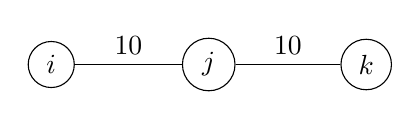
\begin{tikzpicture}
        \node (i) at (-1,0)[circle,draw] {$i$};
        \node (j) at (1,0)[circle,draw] {$j$};
        \node (k) at (3,0)[circle,draw] {$k$};
        \draw (i) -- node[above] {10} (j) -- node[above] {10} (k);
      \end{tikzpicture}
    \end{center}    
  \end{minipage}
  \caption{A network with three agents. Agent $j$ can only split 10
    dollars with either $i$ or $k$, but not both.}
  \label{fig:net-3agents}
\end{SCfigure}

Based on test results, \acro{net} tells us that each person has a
\td{resistance} to each particular payment $p$ given by a resistance
equation.  $i$'s resistance to payment $p$ is given by
\begin{equation}
  \label{eq:resistance}
 r_i = \frac{p_{i}^{\text{max}} - p_i}{p_i - p_i^{\text{con,}}}
\end{equation}
where $p_i^{\text{max}}$ is the maximum $i$ could get and
$p_i^{\text{con}}$ is the no-deal deal. $j$'s resistance is similarly
defined. If we further know that $i$ and $j$ are splitting 10 dollars
then we know that $p_i + p_j = 10$.

\begin{SCfigure}
  \begin{minipage}{1.0\linewidth}
    \begin{center}
      \begin{tikzpicture}[style=dstyle]
        \node (i) at (-1,0)[circle,draw] {$i$};
        \node (j) at (1,0)[circle,draw] {$j$};
        \draw (i) -- node[above] {10} (j);
      \end{tikzpicture}
    \end{center}
  \end{minipage}
  \caption{A sample exchange network with 10 units to be distributed
    among two agents.}
  \label{fig:10}
\end{SCfigure}


The resistance equation is meant to capture the person's resistance to
agreeing to a deal at any particular price. The higher the resistance
the less willing the person is to agree to the deal. Note how this
equation is not linear, as might be expected if people were rational,
but has an exponential shape. This shape tells us a lot about our
irrational behavior.

\acro{net} tells us that exchange happens at the \td{equi-resistance
  point} where both agents have equal resistance, that is where
\begin{equation}
  \label{eq:equi-resistance}
 r_i = \frac{p_{i}^{max} - p_i}{p_i - p_i^{con}} = \frac{p_{j}^{max}
  - p_j}{p_j - p_j^{con}} = r_j. 
\end{equation}

Notice that the equi-resistance equation tells us the agreement that
people will eventually reach via negotiation, but it does not tell us
how the negotiation took place, that is, it does not tell us their
negotiation tactics. 

\begin{SCfigure}
  \begin{minipage}{1.0\linewidth}
  \begin{center}
    \begin{tikzpicture}[style=dstyle]
%      \draw[very thin, color=gray] (-0.1,-0.1) grid (9.9,3.9);
      \draw[->] (-0.1,0) --  node[below] {$p$} (9.9,0);
      \draw[->] (0,-0.1) -- (0,4.5);

      \draw (2,4) node[above] {$r_i(p)$};
      \draw plot[id=ri,domain=2:10] function{(10-x)/x};
      \draw[color=gray] plot[id=rj,domain=0:8] function{x/(10-x)}
      node[above] {\textcolor{black}{$r_j(p)$}};
      \draw[->] (5,4) node[above] {equi-resistance point} --
                (5,1.2) node {};
    \end{tikzpicture}
  \end{center}
  \end{minipage}
  \caption{Resistance of two agents to each possible deal $p$.}
  \label{fig:equi-res}
\end{SCfigure}

We can represent the equi-resistance point graphically by simply
replacing $p_j$ with $10 - p_i$ in $j$'s resistance equation $r_j$ and
plotting the two curves $r_i$ and $r_j$. The point at which the curves
cross is the point of exchange, as shown in figure~\ref{fig:equi-res}.
Of course, the exchange does not always happen at the midpoint. For
example, if $i$ had an offer from some other agent for 6 dollars if it
refused to negotiate with $j$, this would mean that $p_i^{con} = 6$
which would change the equi-resistance point.

%need netlogo model of iterated equi-resistance

We can solve complex \acro{net}s using the \td{iterated
  equi-resistance algorithm}. The algorithm simply uses the
equi-resistance equation repeatedly on each edge of the graph in order
to calculate the payments that these agents can expect to receiver.
This is repeated for all edges until payments stop changing. For
example, for the graph in figure~\ref{fig:net-3agents} we would follow
these steps.

\begin{enumerate}
\item Apply Equi-resistance to
  \begin{tiny}
    \tikz[x=.5cm,y=.5cm]{\node (i) at (-1,0)[circle,draw] {$i$};
      \node (j) at (1,0)[circle,draw] {$j$}; 
      \draw (i) -- node[above] {10} (j);}
  \end{tiny}. Gives us $p_j = 5$.
  
\item Apply Equi-resistance to
  \begin{tiny}
    \tikz[x=.5cm,y=.5cm]{\node (j) at (-1,0)[circle,draw] {$j$};
      \node (k) at (1,0)[circle,draw] {$k$}; 
      \draw (j) -- node[above] {10} (k);}
  \end{tiny}. Let $p_j^{con} = 5$ and apply
  equi-resistance again.
\item Repeat until quiescence.
\end{enumerate}

The iterated equi-resistance algorithm is not guaranteed to converge
and it might converge to different solutions when the edges are sorted
in differently. Even when it does converge the deal it reaches is not
guaranteed to be the one that humans would reach. However, many
experiments have been performed with humans in \emph{small} networks
(less than 12 nodes) which have shown that the iterated
equi-resistance algorithm correctly predicts the resulting deal. This
algorithm gives a new solution for the negotiation problem which,
unlike the solutions in Section~\ref{sec:axiom-solut-conc}, is not
based on some desirable properties of the solution but is based on
evidence from human negotiation, that is, it gives us a descriptive
solution to the negotiation problem. If you want to implement agents that
reach the same solution as humans then you probably want to use the
iterated equi-resistance solution.

\begin{exercises}
\item Given the following utility values for agents $i$ and $j$ over a
  set of possible deals $\delta$:

  \begin{tabular}{lrr} \toprule
    $\delta$ & $u_i(\delta)$ & $u_j(\delta)$ \\ \midrule
    $\delta^1$ & 1 & 0 \\
    $\delta^2$ & 0 & 1 \\
    $\delta^3$ & 1 & 2 \\
    $\delta^4$ & 3 & 1 \\
    $\delta^5$ & 2 & 2 \\
    $\delta^6$ & 1 & 1 \\ 
    $\delta^7$ & 8 & 1 \\ \bottomrule
  \end{tabular}
  \begin{enumerate}
  \item Which deals are on the Pareto frontier?
  \item Which one is the egalitarian social welfare deal?
  \item Which one is the utilitarian deal?
  \item Which one is the Nash bargaining deal?
  \item Which one is the Kalai-Smorodinsky deal?
  \end{enumerate}

\item In a distributed workflow enactment application, a workflow is
  defined as a set of tasks all of which must be performed in order to
  complete the workflow and collect the payment. The following table
  lists the available workflow instances, their tasks and their
  payments:

  \begin{tabular}{{lrr}} \toprule
    Workflow & Tasks & Payment \\ \midrule
    $w_1$ & $t_1, t_1, t_1$ & 6 \\
    $w_2$ & $t_1, t_1, t_2$ & 5 \\
    $w_3$ & $t_1, t_1, t_3$ & 3 \\
    $w_4$ & $t_1, t_2, t_2$ & 1 \\
    $w_5$ & $t_2, t_2, t_3, t_3$ & 8 \\ 
    $w_6$ & $t_2, t_2$ & 1 \\  \bottomrule
  \end{tabular}

  There are three agents. An agent can perform at most two tasks at a
  time, as long as those tasks are \textbf{different}. Also, a task is
  performed for only a single workflow. That, if an agent performs
  $t_1$ for $w_1$ then this $t_1$ cannot be used for any other
  workflow. The goal is for the agents to find the set of workflows
  that maximizes the total payment.

  \begin{enumerate}
  \item Re-state this problem as a negotiation problem, show the set
    of possible deals. (Hint: note that the agents have identical
    capabilities, so you do not need to worry about which one does
    which task).


  \item We further constrain this negotiation by only allowing agents
    to either drop one workflow, add one workflow, or exchange one
    workflow for another. But, they can only do so if this increases
    the total payment (thus, you quickly conclude that they will never
    drop a workflow). Which deals become local optima under these
    constraints?

  \end{enumerate}
\end{exercises}

% Add subaddive cost functions? Postman example is subadditive.

% In Figure 6.15 the agents get more utility for doing a task, instead
% of not doing it. Re-phrase example as costs?

%The NET model has the added advantage that it is a compact way of
%representing multiple parallel negotiations. We can use NETs to show
%all the negotiations that all the agents are involved in at the same.
%But, since NET does not tell us how humans negotiate, only the final
%deal they reach, we still do not know how to program agents to engage
%in these parallel negotiations. A simple solution would be to
%simulate, to some degree, the iterated equi-resistance algorithm but
%run all agents in parallel. We can also try to run multiple instances
%of any one of the negotiation algorithms we have described.


%\section{History}
%\label{sec:history}

%Negotiation has been used for distributed problem solving since the
%beginnings of the field. One of the earliest and most influential
%papers is titled \emph{``Negotiation as a metaphor for distributed
%  problem solving''} \cite{davis83a}---this paper introduced the
%contract-net protocol as a negotiation method.


%Uses taems to set up a complex negotiation problem.
%
% Zhang, Xiaoqin; Lesser, Victor; and Abdallah, Sherief. Efficient
% Management of Multi-Linked Negotiation Based on a Formalized Model.
% Autonomous Agents and Multi-Agent Systems, Volume 10, Number 2, pp.
% 165-205. 2005.



%%% Local Variables: 
%%% mode: latex
%%% TeX-command-default: "PDFlatex"
%%% TeX-master: "~/wp/mas/mas"
%%% End: 
